\documentclass{article}
\usepackage{amsmath}
\usepackage{color,pxfonts,fix-cm}
\usepackage{latexsym}
\usepackage[mathletters]{ucs}
\DeclareUnicodeCharacter{46}{\textperiodcentered}
\DeclareUnicodeCharacter{58}{$\colon$}
\DeclareUnicodeCharacter{8226}{$\bullet$}
\DeclareUnicodeCharacter{60}{\textless}
\DeclareUnicodeCharacter{8217}{\textquoteright}
\DeclareUnicodeCharacter{62}{\textgreater}
\DeclareUnicodeCharacter{8230}{$\ldots$}
\DeclareUnicodeCharacter{32}{$\ $}
\usepackage[T1]{fontenc}
\usepackage[utf8x]{inputenc}
\usepackage{pict2e}
\usepackage{wasysym}
\usepackage[english]{babel}
\usepackage{tikz}
\pagestyle{empty}
\usepackage[margin=0in,paperwidth=960pt,paperheight=540pt]{geometry}
\begin{document}
\definecolor{color_283006}{rgb}{1,1,1}
\definecolor{color_259142}{rgb}{0.905882,0.901961,0.901961}
\definecolor{color_60793}{rgb}{0.109804,0.490196,0.858824}
\definecolor{color_70504}{rgb}{0.160784,0.160784,0.160784}
\definecolor{color_42828}{rgb}{0.043137,0.286275,0.796078}
\definecolor{color_40875}{rgb}{0.035294,0.282353,0.796078}
\definecolor{color_146805}{rgb}{0.462745,0.443137,0.443137}
\begin{tikzpicture}[overlay]
\path(0pt,0pt);
\filldraw[color_283006][even odd rule]
(-15pt, 10pt) -- (944.981pt, 10pt)
 -- (944.981pt, 10pt)
 -- (944.981pt, -529.972pt)
 -- (944.981pt, -529.972pt)
 -- (-15pt, -529.972pt)
 -- (-15pt, -529.972pt)
 -- (-15pt, 10pt) -- cycle
;
\end{tikzpicture}
\begin{picture}(-5,0)(2.5,0)
\put(-15,-529.972){\includegraphics[width=960.0089pt,height=540pt]{latexImage_63a4c9678168f46b4e337841ecdf0595.png}}
\put(62.187,-381.294){\fontsize{28.006}{1}\usefont{T1}{cmr}{m}{n}\selectfont\color{color_259142}Lucas Borges}
\put(62.187,-404.907){\fontsize{18}{1}\usefont{T1}{cmr}{m}{n}\selectfont\color{color_259142}J}
\put(55.072,-92.784){
\includegraphics[width=165.657pt,height=49.521pt]{latexImage_f8368f6ae7995d70866f0f59291f8cf1.png}}
\end{picture}
\newpage
\begin{tikzpicture}[overlay]
\path(0pt,0pt);
\filldraw[color_283006][even odd rule]
(-15pt, 10pt) -- (944.981pt, 10pt)
 -- (944.981pt, 10pt)
 -- (944.981pt, -529.972pt)
 -- (944.981pt, -529.972pt)
 -- (-15pt, -529.972pt)
 -- (-15pt, -529.972pt)
 -- (-15pt, 10pt) -- cycle
;
\end{tikzpicture}
\begin{picture}(-5,0)(2.5,0)
\put(-15,-529.972){
\includegraphics[width=960.009pt,height=540.0001pt]{latexImage_bc4b5025d16a0dea794d2300a0dfe378.png}}
\put(869.806,-486.687){\fontsize{15.987}{1}\usefont{T1}{cmr}{m}{n}\selectfont\color{color_60793}2}
\put(67.687,-180.8){\fontsize{21.997}{1}\usefont{T1}{cmr}{m}{n}\selectfont\color{color_70504}•}
\put(85.687,-181.991){\fontsize{21.997}{1}\usefont{T1}{cmr}{m}{n}\selectfont\color{color_70504}Executive Summary}
\put(67.687,-221.194){\fontsize{21.997}{1}\usefont{T1}{cmr}{m}{n}\selectfont\color{color_70504}•}
\put(85.687,-222.299){\fontsize{21.997}{1}\usefont{T1}{cmr}{m}{n}\selectfont\color{color_70504}Introduction}
\put(67.687,-261.502){\fontsize{21.997}{1}\usefont{T1}{cmr}{m}{n}\selectfont\color{color_70504}•}
\put(85.687,-262.693){\fontsize{21.997}{1}\usefont{T1}{cmr}{m}{n}\selectfont\color{color_70504}Methodology}
\put(67.687,-301.896){\fontsize{21.997}{1}\usefont{T1}{cmr}{m}{n}\selectfont\color{color_70504}•}
\put(85.687,-303.087){\fontsize{21.997}{1}\usefont{T1}{cmr}{m}{n}\selectfont\color{color_70504}Results}
\put(67.687,-342.29){\fontsize{21.997}{1}\usefont{T1}{cmr}{m}{n}\selectfont\color{color_70504}•}
\put(85.687,-343.395){\fontsize{21.997}{1}\usefont{T1}{cmr}{m}{n}\selectfont\color{color_70504}Conclusion}
\put(67.687,-382.598){\fontsize{21.997}{1}\usefont{T1}{cmr}{m}{n}\selectfont\color{color_70504}•}
\put(85.687,-383.789){\fontsize{21.997}{1}\usefont{T1}{cmr}{m}{n}\selectfont\color{color_70504}Appendix}
\put(52.805,-64.69299){\fontsize{33.194}{1}\usefont{T1}{cmr}{m}{n}\selectfont\color{color_42828}Outline}
\end{picture}
\newpage
\begin{tikzpicture}[overlay]
\path(0pt,0pt);
\filldraw[color_283006][even odd rule]
(-15pt, 10pt) -- (944.981pt, 10pt)
 -- (944.981pt, 10pt)
 -- (944.981pt, -529.972pt)
 -- (944.981pt, -529.972pt)
 -- (-15pt, -529.972pt)
 -- (-15pt, -529.972pt)
 -- (-15pt, 10pt) -- cycle
;
\end{tikzpicture}
\begin{picture}(-5,0)(2.5,0)
\put(-15,-529.972){
\includegraphics[width=960.009pt,height=540.0001pt]{latexImage_bc4b5025d16a0dea794d2300a0dfe378.png}}
\put(869.806,-486.687){\fontsize{15.987}{1}\usefont{T1}{cmr}{m}{n}\selectfont\color{color_60793}3}
\put(67.687,-223.49){\fontsize{19.587}{1}\usefont{T1}{cmr}{m}{n}\selectfont\color{color_70504}•}
\put(83.702,-224.51){\fontsize{19.587}{1}\usefont{T1}{cmr}{m}{n}\selectfont\color{color_70504}Summary of methodologies}
\put(67.687,-259.405){\fontsize{19.587}{1}\usefont{T1}{cmr}{m}{n}\selectfont\color{color_70504}•}
\put(83.702,-260.397){\fontsize{19.587}{1}\usefont{T1}{cmr}{m}{n}\selectfont\color{color_70504}Summary of all results}
\put(52.805,-64.69299){\fontsize{33.194}{1}\usefont{T1}{cmr}{m}{n}\selectfont\color{color_42828}Executive Summary}
\end{picture}
\newpage
\begin{tikzpicture}[overlay]
\path(0pt,0pt);
\filldraw[color_283006][even odd rule]
(-15pt, 10pt) -- (944.981pt, 10pt)
 -- (944.981pt, 10pt)
 -- (944.981pt, -529.972pt)
 -- (944.981pt, -529.972pt)
 -- (-15pt, -529.972pt)
 -- (-15pt, -529.972pt)
 -- (-15pt, 10pt) -- cycle
;
\end{tikzpicture}
\begin{picture}(-5,0)(2.5,0)
\put(-15,-529.972){
\includegraphics[width=960.009pt,height=540.0001pt]{latexImage_bc4b5025d16a0dea794d2300a0dfe378.png}}
\put(869.806,-486.687){\fontsize{15.987}{1}\usefont{T1}{cmr}{m}{n}\selectfont\color{color_60793}4}
\put(57.397,-64.69299){\fontsize{33.194}{1}\usefont{T1}{cmr}{m}{n}\selectfont\color{color_42828}Introduction}
\put(67.687,-210.309){\fontsize{21.997}{1}\usefont{T1}{cmr}{m}{n}\selectfont\color{color_70504}•}
\put(85.687,-211.102){\fontsize{21.997}{1}\usefont{T1}{cmr}{m}{n}\selectfont\color{color_70504}Project background and context}
\put(67.687,-248.009){\fontsize{21.997}{1}\usefont{T1}{cmr}{m}{n}\selectfont\color{color_70504}•}
\put(85.687,-248.803){\fontsize{21.997}{1}\usefont{T1}{cmr}{m}{n}\selectfont\color{color_70504}Problems you want to find answers}
\end{picture}
\newpage
\begin{tikzpicture}[overlay]
\path(0pt,0pt);
\filldraw[color_283006][even odd rule]
(-15pt, 10pt) -- (944.981pt, 10pt)
 -- (944.981pt, 10pt)
 -- (944.981pt, -529.972pt)
 -- (944.981pt, -529.972pt)
 -- (-15pt, -529.972pt)
 -- (-15pt, -529.972pt)
 -- (-15pt, 10pt) -- cycle
;
\end{tikzpicture}
\begin{picture}(-5,0)(2.5,0)
\put(-15,-529.972){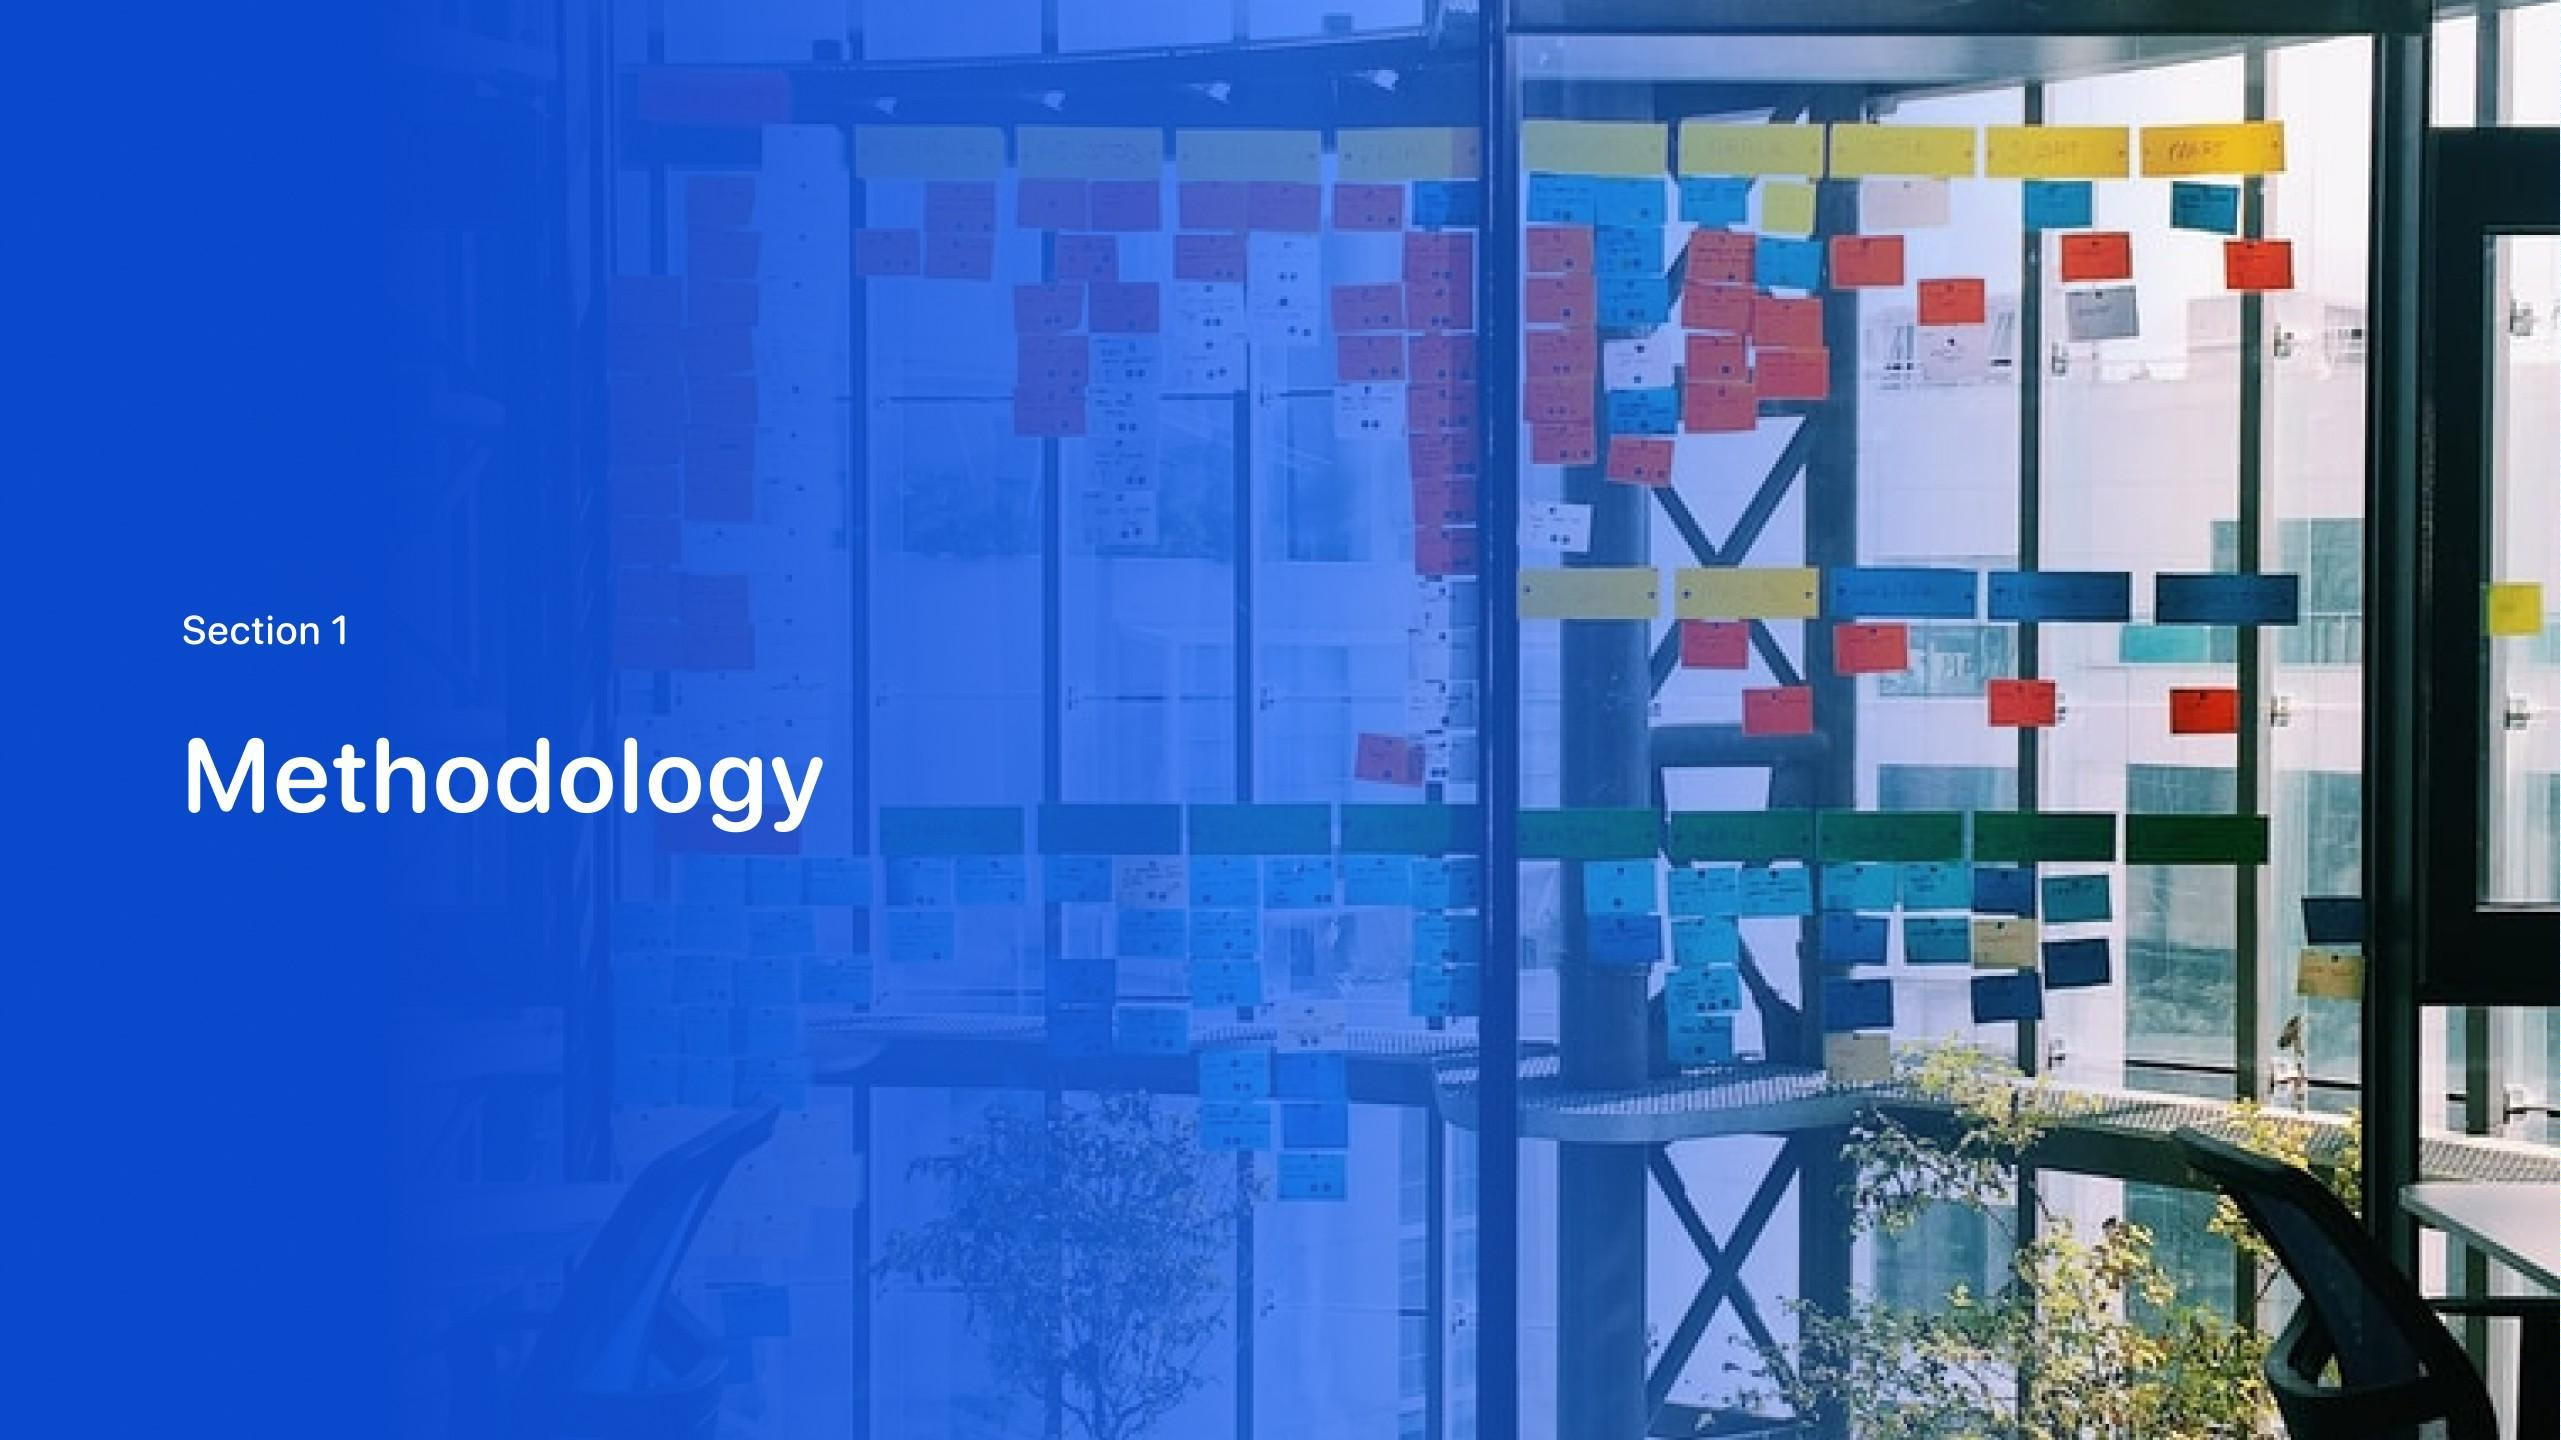
\includegraphics[width=960.009pt,height=540pt]{latexImage_61a8bef55adaa8597655e8bcff41d3f1.png}}
\put(927.605,-511.291){\fontsize{15.987}{1}\usefont{T1}{cmr}{m}{n}\selectfont\color{color_60793}5}
\end{picture}
\begin{tikzpicture}[overlay]
\path(0pt,0pt);
\filldraw[color_40875][even odd rule]
(85.913pt, -240.157pt) -- (45.265pt, -240.157pt)
 -- (45.265pt, -240.157pt)
 -- (45.265pt, -211.443pt)
 -- (45.265pt, -211.443pt)
 -- (126.562pt, -211.443pt)
 -- (126.562pt, -211.443pt)
 -- (126.562pt, -240.157pt)
 -- (126.562pt, -240.157pt)
 -- (85.913pt, -240.157pt) -- cycle
;
\end{tikzpicture}
\begin{picture}(-5,0)(2.5,0)
\put(52.408,-233.014){\fontsize{18}{1}\usefont{T1}{cmr}{m}{n}\selectfont\color{color_283006}Section 1}
\end{picture}
\newpage
\begin{tikzpicture}[overlay]
\path(0pt,0pt);
\filldraw[color_283006][even odd rule]
(-15pt, 10pt) -- (944.981pt, 10pt)
 -- (944.981pt, 10pt)
 -- (944.981pt, -529.972pt)
 -- (944.981pt, -529.972pt)
 -- (-15pt, -529.972pt)
 -- (-15pt, -529.972pt)
 -- (-15pt, 10pt) -- cycle
;
\end{tikzpicture}
\begin{picture}(-5,0)(2.5,0)
\put(-15,-529.972){
\includegraphics[width=960.009pt,height=540.0001pt]{latexImage_bc4b5025d16a0dea794d2300a0dfe378.png}}
\put(869.806,-486.687){\fontsize{15.987}{1}\usefont{T1}{cmr}{m}{n}\selectfont\color{color_60793}6}
\put(52.805,-147.493){\fontsize{23.811}{1}\usefont{T1}{cmr}{m}{n}\selectfont\color{color_42828}Executive Summary}
\put(52.805,-184.088){\fontsize{23.811}{1}\usefont{T1}{cmr}{m}{n}\selectfont\color{color_70504}•}
\put(57.709,-185.392){\fontsize{23.811}{1}\usefont{T1}{cmr}{m}{n}\selectfont\color{color_70504}Data collection methodology:}
\put(62.499,-218.189){\fontsize{20.494}{1}\usefont{T1}{cmr}{m}{n}\selectfont\color{color_146805}•}
\put(67.403,-219.294){\fontsize{20.494}{1}\usefont{T1}{cmr}{m}{n}\selectfont\color{color_146805}Describe how data was collected }
\put(52.805,-255.209){\fontsize{23.811}{1}\usefont{T1}{cmr}{m}{n}\selectfont\color{color_70504}•}
\put(57.709,-256.513){\fontsize{23.811}{1}\usefont{T1}{cmr}{m}{n}\selectfont\color{color_70504}Perform data wrangling}
\put(62.499,-289.31){\fontsize{20.494}{1}\usefont{T1}{cmr}{m}{n}\selectfont\color{color_146805}•}
\put(67.403,-290.387){\fontsize{20.494}{1}\usefont{T1}{cmr}{m}{n}\selectfont\color{color_146805}Describe how data was processed}
\put(52.805,-326.387){\fontsize{23.811}{1}\usefont{T1}{cmr}{m}{n}\selectfont\color{color_70504}•}
\put(57.709,-327.691){\fontsize{23.811}{1}\usefont{T1}{cmr}{m}{n}\selectfont\color{color_70504}Perform exploratory data analysis (EDA) using visualization }
\put(57.709,-361.792){\fontsize{23.811}{1}\usefont{T1}{cmr}{m}{n}\selectfont\color{color_70504}and SQL}
\put(52.805,-398.387){\fontsize{23.811}{1}\usefont{T1}{cmr}{m}{n}\selectfont\color{color_70504}•}
\put(57.709,-399.691){\fontsize{23.811}{1}\usefont{T1}{cmr}{m}{n}\selectfont\color{color_70504}Perform interactive visual analytics using Folium and Plotly Dash}
\put(52.805,-436.287){\fontsize{23.811}{1}\usefont{T1}{cmr}{m}{n}\selectfont\color{color_70504}•}
\put(57.709,-437.591){\fontsize{23.811}{1}\usefont{T1}{cmr}{m}{n}\selectfont\color{color_70504}Perform predictive analysis using classification models}
\put(62.499,-470.387){\fontsize{20.494}{1}\usefont{T1}{cmr}{m}{n}\selectfont\color{color_146805}•}
\put(67.403,-471.493){\fontsize{20.494}{1}\usefont{T1}{cmr}{m}{n}\selectfont\color{color_146805}How to build, tune, evaluate classification models}
\put(52.805,-64.69299){\fontsize{33.194}{1}\usefont{T1}{cmr}{m}{n}\selectfont\color{color_42828}Methodology}
\end{picture}
\newpage
\begin{tikzpicture}[overlay]
\path(0pt,0pt);
\filldraw[color_283006][even odd rule]
(-15pt, 10pt) -- (944.981pt, 10pt)
 -- (944.981pt, 10pt)
 -- (944.981pt, -529.972pt)
 -- (944.981pt, -529.972pt)
 -- (-15pt, -529.972pt)
 -- (-15pt, -529.972pt)
 -- (-15pt, 10pt) -- cycle
;
\end{tikzpicture}
\begin{picture}(-5,0)(2.5,0)
\put(-15,-529.972){
\includegraphics[width=960.009pt,height=540.0001pt]{latexImage_bc4b5025d16a0dea794d2300a0dfe378.png}}
\put(869.806,-486.687){\fontsize{15.987}{1}\usefont{T1}{cmr}{m}{n}\selectfont\color{color_60793}7}
\put(52.691,-159.313){\fontsize{21.997}{1}\usefont{T1}{cmr}{m}{n}\selectfont\color{color_70504}Describe how data sets were collected. }
\put(52.691,-199.707){\fontsize{21.997}{1}\usefont{T1}{cmr}{m}{n}\selectfont\color{color_70504}You need to present your data collection process use key phrases and }
\put(52.691,-226.098){\fontsize{21.997}{1}\usefont{T1}{cmr}{m}{n}\selectfont\color{color_70504}flowcharts}
\put(52.805,-64.69299){\fontsize{33.194}{1}\usefont{T1}{cmr}{m}{n}\selectfont\color{color_42828}Data Collection}
\end{picture}
\newpage
\begin{tikzpicture}[overlay]
\path(0pt,0pt);
\filldraw[color_283006][even odd rule]
(-15pt, 10pt) -- (944.981pt, 10pt)
 -- (944.981pt, 10pt)
 -- (944.981pt, -529.972pt)
 -- (944.981pt, -529.972pt)
 -- (-15pt, -529.972pt)
 -- (-15pt, -529.972pt)
 -- (-15pt, 10pt) -- cycle
;
\end{tikzpicture}
\begin{picture}(-5,0)(2.5,0)
\put(-15,-529.972){
\includegraphics[width=960.009pt,height=540.0001pt]{latexImage_bc4b5025d16a0dea794d2300a0dfe378.png}}
\put(869.806,-486.687){\fontsize{15.987}{1}\usefont{T1}{cmr}{m}{n}\selectfont\color{color_60793}8}
\end{picture}
\begin{tikzpicture}[overlay]
\path(0pt,0pt);
\draw[color_42828,line width=1pt,dash pattern=on 3.05569pt off 2.29177pt,line join=round]
(665.343pt, -462.365pt) -- (450.364pt, -462.365pt)
 -- (450.364pt, -462.365pt)
 -- (450.364pt, -131.137pt)
 -- (450.364pt, -131.137pt)
 -- (880.323pt, -131.137pt)
 -- (880.323pt, -131.137pt)
 -- (880.323pt, -462.365pt)
 -- (880.323pt, -462.365pt)
 -- (665.343pt, -462.365pt) -- cycle
;
\end{tikzpicture}
\begin{picture}(-5,0)(2.5,0)
\put(457.592,-262.211){\fontsize{21.997}{1}\usefont{T1}{cmr}{m}{n}\selectfont\color{color_60793}Place your flowchart of SpaceX API }
\put(457.592,-288.488){\fontsize{21.997}{1}\usefont{T1}{cmr}{m}{n}\selectfont\color{color_60793}calls here}
\put(56.802,-156.195){\fontsize{21.997}{1}\usefont{T1}{cmr}{m}{n}\selectfont\color{color_70504}•}
\put(74.802,-157.301){\fontsize{21.997}{1}\usefont{T1}{cmr}{m}{n}\selectfont\color{color_70504}Present your data collection }
\put(74.802,-183.691){\fontsize{21.997}{1}\usefont{T1}{cmr}{m}{n}\selectfont\color{color_70504}with SpaceX REST calls using }
\put(74.802,-210.11){\fontsize{21.997}{1}\usefont{T1}{cmr}{m}{n}\selectfont\color{color_70504}key phrases and flowcharts}
\put(56.802,-289.594){\fontsize{21.997}{1}\usefont{T1}{cmr}{m}{n}\selectfont\color{color_70504}•}
\put(74.802,-290.813){\fontsize{21.997}{1}\usefont{T1}{cmr}{m}{n}\selectfont\color{color_70504}Add the GitHub URL of the }
\put(74.802,-317.09){\fontsize{21.997}{1}\usefont{T1}{cmr}{m}{n}\selectfont\color{color_70504}completed SpaceX API calls }
\put(74.802,-343.509){\fontsize{21.997}{1}\usefont{T1}{cmr}{m}{n}\selectfont\color{color_70504}notebook (must include }
\put(74.802,-369.899){\fontsize{21.997}{1}\usefont{T1}{cmr}{m}{n}\selectfont\color{color_60793}completed code cell and }
\put(74.802,-396.205){\fontsize{21.997}{1}\usefont{T1}{cmr}{m}{n}\selectfont\color{color_60793}outcome cell), as an external }
\put(74.802,-422.595){\fontsize{21.997}{1}\usefont{T1}{cmr}{m}{n}\selectfont\color{color_70504}reference and peer-review }
\put(74.802,-449.014){\fontsize{21.997}{1}\usefont{T1}{cmr}{m}{n}\selectfont\color{color_70504}purpose}
\put(52.805,-64.69299){\fontsize{33.194}{1}\usefont{T1}{cmr}{m}{n}\selectfont\color{color_42828}Data Collection – SpaceX API}
\end{picture}
\newpage
\begin{tikzpicture}[overlay]
\path(0pt,0pt);
\filldraw[color_283006][even odd rule]
(-15pt, 10pt) -- (944.981pt, 10pt)
 -- (944.981pt, 10pt)
 -- (944.981pt, -529.972pt)
 -- (944.981pt, -529.972pt)
 -- (-15pt, -529.972pt)
 -- (-15pt, -529.972pt)
 -- (-15pt, 10pt) -- cycle
;
\end{tikzpicture}
\begin{picture}(-5,0)(2.5,0)
\put(-15,-529.972){
\includegraphics[width=960.009pt,height=540.0001pt]{latexImage_bc4b5025d16a0dea794d2300a0dfe378.png}}
\put(869.806,-486.687){\fontsize{15.987}{1}\usefont{T1}{cmr}{m}{n}\selectfont\color{color_60793}9}
\put(64.795,-155.487){\fontsize{21.997}{1}\usefont{T1}{cmr}{m}{n}\selectfont\color{color_70504}•}
\put(82.795,-156.706){\fontsize{21.997}{1}\usefont{T1}{cmr}{m}{n}\selectfont\color{color_70504}Present your web }
\put(82.795,-183.096){\fontsize{21.997}{1}\usefont{T1}{cmr}{m}{n}\selectfont\color{color_70504}scraping process using }
\put(82.795,-209.487){\fontsize{21.997}{1}\usefont{T1}{cmr}{m}{n}\selectfont\color{color_70504}key phrases and }
\put(82.795,-235.906){\fontsize{21.997}{1}\usefont{T1}{cmr}{m}{n}\selectfont\color{color_70504}flowcharts}
\put(64.795,-315.502){\fontsize{21.997}{1}\usefont{T1}{cmr}{m}{n}\selectfont\color{color_70504}•}
\put(82.795,-316.693){\fontsize{21.997}{1}\usefont{T1}{cmr}{m}{n}\selectfont\color{color_70504}Add the GitHub URL of }
\put(82.795,-343.112){\fontsize{21.997}{1}\usefont{T1}{cmr}{m}{n}\selectfont\color{color_70504}the completed web }
\put(82.795,-369.502){\fontsize{21.997}{1}\usefont{T1}{cmr}{m}{n}\selectfont\color{color_70504}scraping notebook, as an }
\put(82.795,-395.893){\fontsize{21.997}{1}\usefont{T1}{cmr}{m}{n}\selectfont\color{color_70504}external reference and }
\put(82.795,-422.312){\fontsize{21.997}{1}\usefont{T1}{cmr}{m}{n}\selectfont\color{color_70504}peer-review purpose}
\put(64.795,-76.797){\fontsize{33.194}{1}\usefont{T1}{cmr}{m}{n}\selectfont\color{color_42828}Data Collection - Scraping}
\end{picture}
\begin{tikzpicture}[overlay]
\path(0pt,0pt);
\draw[color_42828,line width=1pt,dash pattern=on 3.05569pt off 2.29177pt,line join=round]
(665.343pt, -462.337pt) -- (450.364pt, -462.337pt)
 -- (450.364pt, -462.337pt)
 -- (450.364pt, -131.109pt)
 -- (450.364pt, -131.109pt)
 -- (880.323pt, -131.109pt)
 -- (880.323pt, -131.109pt)
 -- (880.323pt, -462.337pt)
 -- (880.323pt, -462.337pt)
 -- (665.343pt, -462.337pt) -- cycle
;
\end{tikzpicture}
\begin{picture}(-5,0)(2.5,0)
\put(457.592,-291.209){\fontsize{21.997}{1}\usefont{T1}{cmr}{m}{n}\selectfont\color{color_60793}Place your flowchart of web scraping }
\put(457.592,-314.992){\fontsize{21.997}{1}\usefont{T1}{cmr}{m}{n}\selectfont\color{color_60793}here}
\end{picture}
\newpage
\begin{tikzpicture}[overlay]
\path(0pt,0pt);
\filldraw[color_283006][even odd rule]
(-15pt, 10pt) -- (944.981pt, 10pt)
 -- (944.981pt, 10pt)
 -- (944.981pt, -529.972pt)
 -- (944.981pt, -529.972pt)
 -- (-15pt, -529.972pt)
 -- (-15pt, -529.972pt)
 -- (-15pt, 10pt) -- cycle
;
\end{tikzpicture}
\begin{picture}(-5,0)(2.5,0)
\put(-15,-529.972){
\includegraphics[width=960.009pt,height=540.0001pt]{latexImage_bc4b5025d16a0dea794d2300a0dfe378.png}}
\put(859.602,-486.687){\fontsize{15.987}{1}\usefont{T1}{cmr}{m}{n}\selectfont\color{color_60793}10}
\put(52.691,-159.313){\fontsize{21.997}{1}\usefont{T1}{cmr}{m}{n}\selectfont\color{color_70504}Describe how data were processed}
\put(52.691,-185.704){\fontsize{21.997}{1}\usefont{T1}{cmr}{m}{n}\selectfont\color{color_70504}You need to present your data wrangling process using key }
\put(52.691,-212.094){\fontsize{21.997}{1}\usefont{T1}{cmr}{m}{n}\selectfont\color{color_70504}phrases and flowcharts}
\put(52.691,-238.513){\fontsize{21.997}{1}\usefont{T1}{cmr}{m}{n}\selectfont\color{color_70504}Add the GitHub URL of your completed data wrangling related }
\put(52.691,-264.791){\fontsize{21.997}{1}\usefont{T1}{cmr}{m}{n}\selectfont\color{color_70504}notebooks, as an external reference and peer-review purpose}
\put(52.805,-64.69299){\fontsize{33.194}{1}\usefont{T1}{cmr}{m}{n}\selectfont\color{color_42828}Data Wrangling}
\end{picture}
\newpage
\begin{tikzpicture}[overlay]
\path(0pt,0pt);
\filldraw[color_283006][even odd rule]
(-15pt, 10pt) -- (944.981pt, 10pt)
 -- (944.981pt, 10pt)
 -- (944.981pt, -529.972pt)
 -- (944.981pt, -529.972pt)
 -- (-15pt, -529.972pt)
 -- (-15pt, -529.972pt)
 -- (-15pt, 10pt) -- cycle
;
\end{tikzpicture}
\begin{picture}(-5,0)(2.5,0)
\put(-15,-529.972){
\includegraphics[width=960.009pt,height=540.0001pt]{latexImage_bc4b5025d16a0dea794d2300a0dfe378.png}}
\put(859.602,-486.687){\fontsize{15.987}{1}\usefont{T1}{cmr}{m}{n}\selectfont\color{color_60793}11}
\put(52.805,-159.313){\fontsize{21.997}{1}\usefont{T1}{cmr}{m}{n}\selectfont\color{color_70504}Summarize what charts were plotted and why you used those }
\put(52.805,-185.704){\fontsize{21.997}{1}\usefont{T1}{cmr}{m}{n}\selectfont\color{color_70504}charts}
\put(52.805,-226.098){\fontsize{21.997}{1}\usefont{T1}{cmr}{m}{n}\selectfont\color{color_70504}Add the GitHub URL of your completed EDA with data visualization }
\put(52.805,-252.488){\fontsize{21.997}{1}\usefont{T1}{cmr}{m}{n}\selectfont\color{color_70504}notebook, as an external reference and peer-review purpose}
\put(52.805,-64.69299){\fontsize{33.194}{1}\usefont{T1}{cmr}{m}{n}\selectfont\color{color_42828}EDA with Data Visualization}
\end{picture}
\newpage
\begin{tikzpicture}[overlay]
\path(0pt,0pt);
\filldraw[color_283006][even odd rule]
(-15pt, 10pt) -- (944.981pt, 10pt)
 -- (944.981pt, 10pt)
 -- (944.981pt, -529.972pt)
 -- (944.981pt, -529.972pt)
 -- (-15pt, -529.972pt)
 -- (-15pt, -529.972pt)
 -- (-15pt, 10pt) -- cycle
;
\end{tikzpicture}
\begin{picture}(-5,0)(2.5,0)
\put(-15,-529.972){
\includegraphics[width=960.009pt,height=540.0001pt]{latexImage_bc4b5025d16a0dea794d2300a0dfe378.png}}
\put(859.602,-486.687){\fontsize{15.987}{1}\usefont{T1}{cmr}{m}{n}\selectfont\color{color_60793}12}
\put(52.805,-157.811){\fontsize{21.997}{1}\usefont{T1}{cmr}{m}{n}\selectfont\color{color_70504}Using bullet point format, summarize the SQL queries you }
\put(52.805,-184.202){\fontsize{21.997}{1}\usefont{T1}{cmr}{m}{n}\selectfont\color{color_70504}performed}
\put(52.805,-224.595){\fontsize{21.997}{1}\usefont{T1}{cmr}{m}{n}\selectfont\color{color_70504}Add the GitHub URL of your completed EDA with SQL notebook, as }
\put(52.805,-251.014){\fontsize{21.997}{1}\usefont{T1}{cmr}{m}{n}\selectfont\color{color_70504}an external reference and peer-review purpose}
\put(52.805,-64.69299){\fontsize{33.194}{1}\usefont{T1}{cmr}{m}{n}\selectfont\color{color_42828}EDA with SQL}
\end{picture}
\newpage
\begin{tikzpicture}[overlay]
\path(0pt,0pt);
\filldraw[color_283006][even odd rule]
(-15pt, 10pt) -- (944.981pt, 10pt)
 -- (944.981pt, 10pt)
 -- (944.981pt, -529.972pt)
 -- (944.981pt, -529.972pt)
 -- (-15pt, -529.972pt)
 -- (-15pt, -529.972pt)
 -- (-15pt, 10pt) -- cycle
;
\end{tikzpicture}
\begin{picture}(-5,0)(2.5,0)
\put(-15,-529.972){
\includegraphics[width=960.009pt,height=540.0001pt]{latexImage_bc4b5025d16a0dea794d2300a0dfe378.png}}
\put(859.602,-486.687){\fontsize{15.987}{1}\usefont{T1}{cmr}{m}{n}\selectfont\color{color_60793}13}
\put(58.106,-163.112){\fontsize{21.997}{1}\usefont{T1}{cmr}{m}{n}\selectfont\color{color_70504}Summarize what map objects such as markers, circles, lines, etc. you }
\put(58.106,-189.502){\fontsize{21.997}{1}\usefont{T1}{cmr}{m}{n}\selectfont\color{color_70504}created and added to a folium map}
\put(58.106,-229.896){\fontsize{21.997}{1}\usefont{T1}{cmr}{m}{n}\selectfont\color{color_70504}Explain why you added those objects}
\put(58.106,-270.205){\fontsize{21.997}{1}\usefont{T1}{cmr}{m}{n}\selectfont\color{color_70504}Add the GitHub URL of your completed interactive map with Folium map, }
\put(58.106,-296.595){\fontsize{21.997}{1}\usefont{T1}{cmr}{m}{n}\selectfont\color{color_70504}as an external reference and peer-review purpose}
\put(52.805,-64.69299){\fontsize{33.194}{1}\usefont{T1}{cmr}{m}{n}\selectfont\color{color_42828}Build an Interactive Map with Folium}
\end{picture}
\newpage
\begin{tikzpicture}[overlay]
\path(0pt,0pt);
\filldraw[color_283006][even odd rule]
(-15pt, 10pt) -- (944.981pt, 10pt)
 -- (944.981pt, 10pt)
 -- (944.981pt, -529.972pt)
 -- (944.981pt, -529.972pt)
 -- (-15pt, -529.972pt)
 -- (-15pt, -529.972pt)
 -- (-15pt, 10pt) -- cycle
;
\end{tikzpicture}
\begin{picture}(-5,0)(2.5,0)
\put(-15,-529.972){
\includegraphics[width=960.009pt,height=540.0001pt]{latexImage_bc4b5025d16a0dea794d2300a0dfe378.png}}
\put(859.602,-486.687){\fontsize{15.987}{1}\usefont{T1}{cmr}{m}{n}\selectfont\color{color_60793}14}
\put(52.805,-159.313){\fontsize{21.997}{1}\usefont{T1}{cmr}{m}{n}\selectfont\color{color_70504}Summarize what plots/graphs and interactions you have added to a }
\put(52.805,-185.704){\fontsize{21.997}{1}\usefont{T1}{cmr}{m}{n}\selectfont\color{color_70504}dashboard}
\put(52.805,-226.013){\fontsize{21.997}{1}\usefont{T1}{cmr}{m}{n}\selectfont\color{color_70504}Explain why you added those plots and interactions}
\put(52.805,-266.406){\fontsize{21.997}{1}\usefont{T1}{cmr}{m}{n}\selectfont\color{color_70504}Add the GitHub URL of your completed Plotly Dash lab, as an }
\put(52.805,-292.797){\fontsize{21.997}{1}\usefont{T1}{cmr}{m}{n}\selectfont\color{color_70504}external reference and peer-review purpose}
\put(52.805,-64.69299){\fontsize{33.194}{1}\usefont{T1}{cmr}{m}{n}\selectfont\color{color_42828}Build a Dashboard with Plotly Dash}
\end{picture}
\newpage
\begin{tikzpicture}[overlay]
\path(0pt,0pt);
\filldraw[color_283006][even odd rule]
(-15pt, 10pt) -- (944.981pt, 10pt)
 -- (944.981pt, 10pt)
 -- (944.981pt, -529.972pt)
 -- (944.981pt, -529.972pt)
 -- (-15pt, -529.972pt)
 -- (-15pt, -529.972pt)
 -- (-15pt, 10pt) -- cycle
;
\end{tikzpicture}
\begin{picture}(-5,0)(2.5,0)
\put(-15,-529.972){
\includegraphics[width=960.009pt,height=540.0001pt]{latexImage_bc4b5025d16a0dea794d2300a0dfe378.png}}
\put(859.602,-486.687){\fontsize{15.987}{1}\usefont{T1}{cmr}{m}{n}\selectfont\color{color_60793}15}
\put(52.691,-159.313){\fontsize{21.997}{1}\usefont{T1}{cmr}{m}{n}\selectfont\color{color_70504}Summarize how you built, evaluated, improved, and found the best }
\put(52.691,-185.591){\fontsize{21.997}{1}\usefont{T1}{cmr}{m}{n}\selectfont\color{color_70504}performing classification model}
\put(52.691,-226.013){\fontsize{21.997}{1}\usefont{T1}{cmr}{m}{n}\selectfont\color{color_70504}You need present your model development process using key }
\put(52.691,-252.29){\fontsize{21.997}{1}\usefont{T1}{cmr}{m}{n}\selectfont\color{color_70504}phrases and flowchart}
\put(52.691,-292.712){\fontsize{21.997}{1}\usefont{T1}{cmr}{m}{n}\selectfont\color{color_70504}Add the GitHub URL of your completed predictive analysis lab, as an }
\put(52.691,-319.102){\fontsize{21.997}{1}\usefont{T1}{cmr}{m}{n}\selectfont\color{color_70504}external reference and peer-review purpose}
\put(52.805,-64.69299){\fontsize{33.194}{1}\usefont{T1}{cmr}{m}{n}\selectfont\color{color_42828}Predictive Analysis (Classification)}
\end{picture}
\newpage
\begin{tikzpicture}[overlay]
\path(0pt,0pt);
\filldraw[color_283006][even odd rule]
(-15pt, 10pt) -- (944.981pt, 10pt)
 -- (944.981pt, 10pt)
 -- (944.981pt, -529.972pt)
 -- (944.981pt, -529.972pt)
 -- (-15pt, -529.972pt)
 -- (-15pt, -529.972pt)
 -- (-15pt, 10pt) -- cycle
;
\end{tikzpicture}
\begin{picture}(-5,0)(2.5,0)
\put(-15,-529.972){
\includegraphics[width=960.009pt,height=540.0001pt]{latexImage_bc4b5025d16a0dea794d2300a0dfe378.png}}
\put(859.602,-486.687){\fontsize{15.987}{1}\usefont{T1}{cmr}{m}{n}\selectfont\color{color_60793}16}
\put(58.389,-156.706){\fontsize{21.997}{1}\usefont{T1}{cmr}{m}{n}\selectfont\color{color_70504}•}
\put(76.389,-157.896){\fontsize{21.997}{1}\usefont{T1}{cmr}{m}{n}\selectfont\color{color_70504}Exploratory data analysis results}
\put(58.389,-197.099){\fontsize{21.997}{1}\usefont{T1}{cmr}{m}{n}\selectfont\color{color_70504}•}
\put(76.389,-198.205){\fontsize{21.997}{1}\usefont{T1}{cmr}{m}{n}\selectfont\color{color_70504}Interactive analytics demo in screenshots}
\put(58.389,-237.408){\fontsize{21.997}{1}\usefont{T1}{cmr}{m}{n}\selectfont\color{color_70504}•}
\put(76.389,-238.598){\fontsize{21.997}{1}\usefont{T1}{cmr}{m}{n}\selectfont\color{color_70504}Predictive analysis results}
\put(52.805,-64.69299){\fontsize{33.194}{1}\usefont{T1}{cmr}{m}{n}\selectfont\color{color_42828}Results}
\end{picture}
\newpage
\begin{tikzpicture}[overlay]
\path(0pt,0pt);
\filldraw[color_283006][even odd rule]
(-15pt, 10pt) -- (944.981pt, 10pt)
 -- (944.981pt, 10pt)
 -- (944.981pt, -529.972pt)
 -- (944.981pt, -529.972pt)
 -- (-15pt, -529.972pt)
 -- (-15pt, -529.972pt)
 -- (-15pt, 10pt) -- cycle
;
\end{tikzpicture}
\begin{picture}(-5,0)(2.5,0)
\put(-15,-529.972){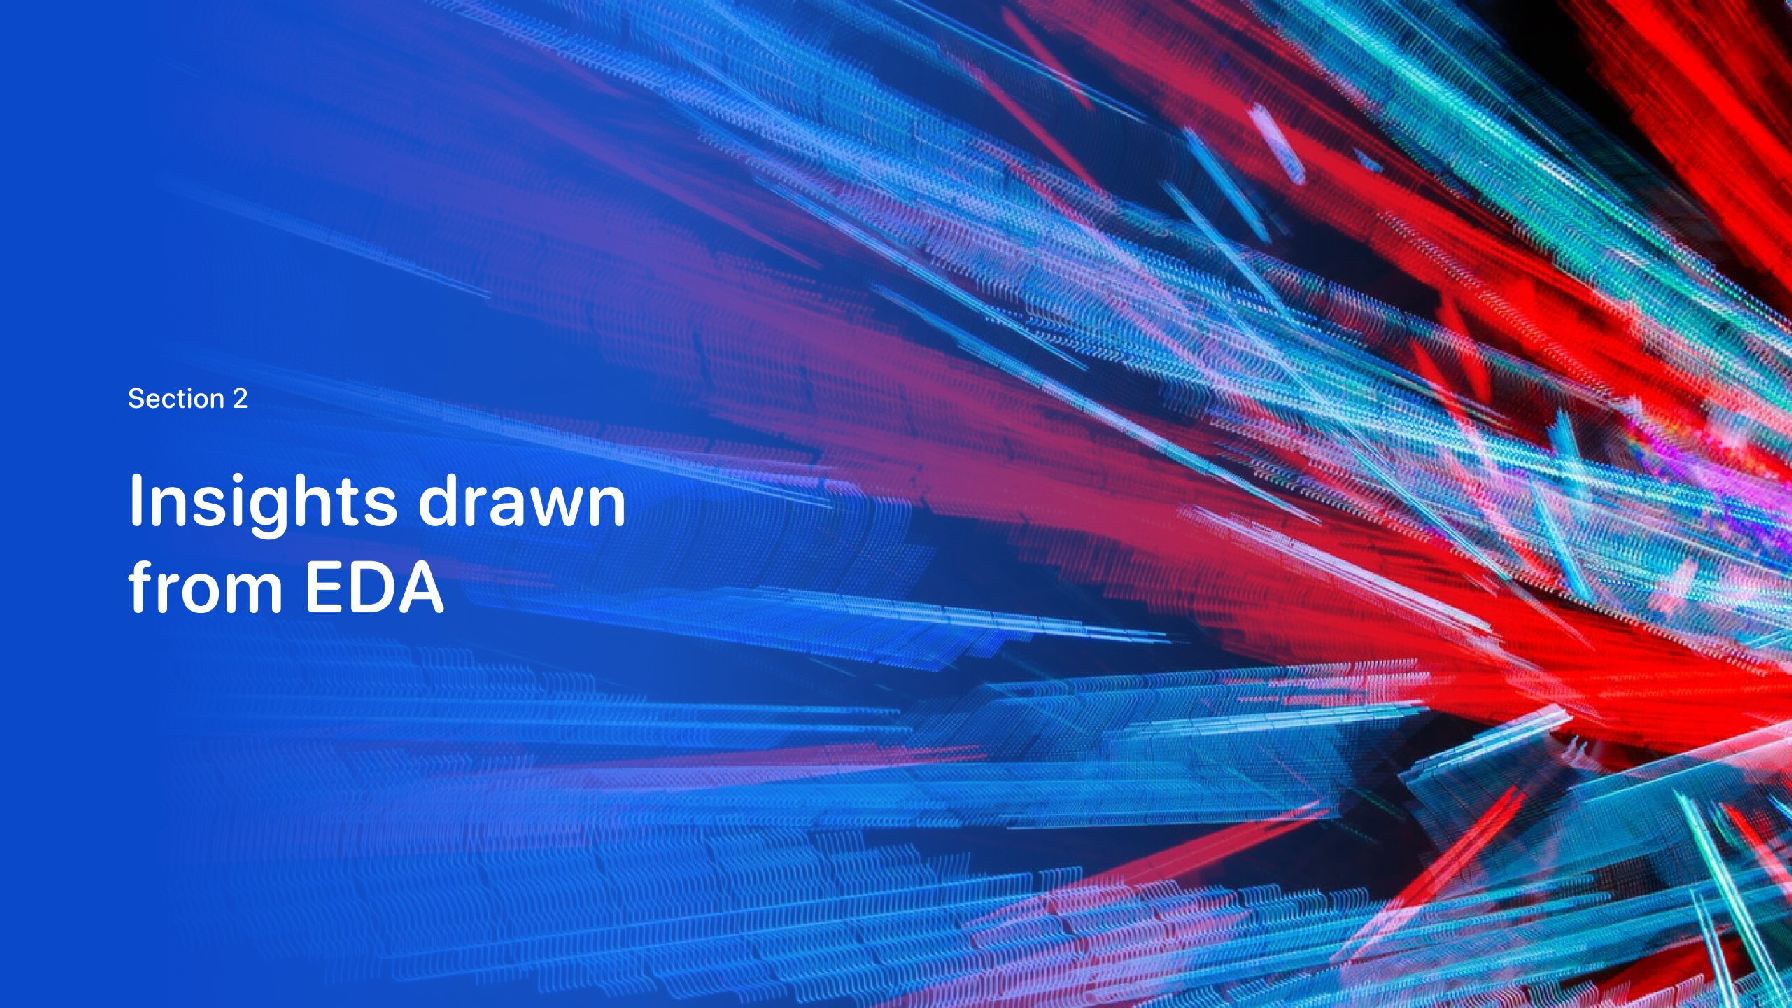
\includegraphics[width=960.009pt,height=540.0001pt]{latexImage_ab239b8be2bdb5212c69bade20de7b36.png}}
\end{picture}
\begin{tikzpicture}[overlay]
\path(0pt,0pt);
\filldraw[color_40875][even odd rule]
(88.493pt, -217.877pt) -- (47.844pt, -217.877pt)
 -- (47.844pt, -217.877pt)
 -- (47.844pt, -189.162pt)
 -- (47.844pt, -189.162pt)
 -- (129.142pt, -189.162pt)
 -- (129.142pt, -189.162pt)
 -- (129.142pt, -217.877pt)
 -- (129.142pt, -217.877pt)
 -- (88.493pt, -217.877pt) -- cycle
;
\end{tikzpicture}
\begin{picture}(-5,0)(2.5,0)
\put(54.902,-210.706){\fontsize{18}{1}\usefont{T1}{cmr}{m}{n}\selectfont\color{color_283006}Section 2}
\end{picture}
\newpage
\begin{tikzpicture}[overlay]
\path(0pt,0pt);
\filldraw[color_283006][even odd rule]
(-15pt, 10pt) -- (944.981pt, 10pt)
 -- (944.981pt, 10pt)
 -- (944.981pt, -529.972pt)
 -- (944.981pt, -529.972pt)
 -- (-15pt, -529.972pt)
 -- (-15pt, -529.972pt)
 -- (-15pt, 10pt) -- cycle
;
\end{tikzpicture}
\begin{picture}(-5,0)(2.5,0)
\put(-15,-529.972){
\includegraphics[width=960.009pt,height=540.0001pt]{latexImage_bc4b5025d16a0dea794d2300a0dfe378.png}}
\put(859.602,-486.687){\fontsize{15.987}{1}\usefont{T1}{cmr}{m}{n}\selectfont\color{color_60793}18}
\put(60.203,-176.293){\fontsize{21.997}{1}\usefont{T1}{cmr}{m}{n}\selectfont\color{color_70504}•}
\put(78.203,-177.512){\fontsize{21.997}{1}\usefont{T1}{cmr}{m}{n}\selectfont\color{color_70504}Show a scatter plot }
\put(78.203,-203.902){\fontsize{21.997}{1}\usefont{T1}{cmr}{m}{n}\selectfont\color{color_70504}of Flight Number vs. }
\put(78.203,-230.208){\fontsize{21.997}{1}\usefont{T1}{cmr}{m}{n}\selectfont\color{color_70504}Launch Site}
\put(60.203,-309.805){\fontsize{21.997}{1}\usefont{T1}{cmr}{m}{n}\selectfont\color{color_70504}•}
\put(78.203,-310.995){\fontsize{21.997}{1}\usefont{T1}{cmr}{m}{n}\selectfont\color{color_70504}Show the screenshot of }
\put(78.203,-337.301){\fontsize{21.997}{1}\usefont{T1}{cmr}{m}{n}\selectfont\color{color_70504}the scatter plot with }
\put(78.203,-363.691){\fontsize{21.997}{1}\usefont{T1}{cmr}{m}{n}\selectfont\color{color_70504}explanations}
\put(52.805,-64.69299){\fontsize{33.194}{1}\usefont{T1}{cmr}{m}{n}\selectfont\color{color_42828}Flight Number vs. Launch Site}
\end{picture}
\newpage
\begin{tikzpicture}[overlay]
\path(0pt,0pt);
\filldraw[color_283006][even odd rule]
(-15pt, 10pt) -- (944.981pt, 10pt)
 -- (944.981pt, 10pt)
 -- (944.981pt, -529.972pt)
 -- (944.981pt, -529.972pt)
 -- (-15pt, -529.972pt)
 -- (-15pt, -529.972pt)
 -- (-15pt, 10pt) -- cycle
;
\end{tikzpicture}
\begin{picture}(-5,0)(2.5,0)
\put(-15,-529.972){
\includegraphics[width=960.009pt,height=540.0001pt]{latexImage_bc4b5025d16a0dea794d2300a0dfe378.png}}
\put(859.602,-486.687){\fontsize{15.987}{1}\usefont{T1}{cmr}{m}{n}\selectfont\color{color_60793}19}
\put(52.691,-177.313){\fontsize{21.997}{1}\usefont{T1}{cmr}{m}{n}\selectfont\color{color_70504}•}
\put(70.691,-178.504){\fontsize{21.997}{1}\usefont{T1}{cmr}{m}{n}\selectfont\color{color_70504}Show a scatter plot }
\put(70.691,-204.809){\fontsize{21.997}{1}\usefont{T1}{cmr}{m}{n}\selectfont\color{color_70504}of Payload vs. Launch }
\put(70.691,-231.2){\fontsize{21.997}{1}\usefont{T1}{cmr}{m}{n}\selectfont\color{color_70504}Site}
\put(52.691,-310.797){\fontsize{21.997}{1}\usefont{T1}{cmr}{m}{n}\selectfont\color{color_70504}•}
\put(70.691,-311.902){\fontsize{21.997}{1}\usefont{T1}{cmr}{m}{n}\selectfont\color{color_70504}Show the screenshot of }
\put(70.691,-338.293){\fontsize{21.997}{1}\usefont{T1}{cmr}{m}{n}\selectfont\color{color_70504}the scatter plot with }
\put(70.691,-364.712){\fontsize{21.997}{1}\usefont{T1}{cmr}{m}{n}\selectfont\color{color_70504}explanations}
\put(52.805,-64.69299){\fontsize{33.194}{1}\usefont{T1}{cmr}{m}{n}\selectfont\color{color_42828}Payload vs. Launch Site}
\end{picture}
\newpage
\begin{tikzpicture}[overlay]
\path(0pt,0pt);
\filldraw[color_283006][even odd rule]
(-15pt, 10pt) -- (944.981pt, 10pt)
 -- (944.981pt, 10pt)
 -- (944.981pt, -529.972pt)
 -- (944.981pt, -529.972pt)
 -- (-15pt, -529.972pt)
 -- (-15pt, -529.972pt)
 -- (-15pt, 10pt) -- cycle
;
\end{tikzpicture}
\begin{picture}(-5,0)(2.5,0)
\put(-15,-529.972){
\includegraphics[width=960.009pt,height=540.0001pt]{latexImage_bc4b5025d16a0dea794d2300a0dfe378.png}}
\put(859.602,-486.687){\fontsize{15.987}{1}\usefont{T1}{cmr}{m}{n}\selectfont\color{color_60793}20}
\put(52.691,-178.306){\fontsize{21.997}{1}\usefont{T1}{cmr}{m}{n}\selectfont\color{color_70504}•}
\put(70.691,-179.496){\fontsize{21.997}{1}\usefont{T1}{cmr}{m}{n}\selectfont\color{color_70504}Show a bar chart for the }
\put(70.691,-205.802){\fontsize{21.997}{1}\usefont{T1}{cmr}{m}{n}\selectfont\color{color_70504}success rate of each }
\put(70.691,-232.192){\fontsize{21.997}{1}\usefont{T1}{cmr}{m}{n}\selectfont\color{color_70504}orbit type}
\put(52.691,-311.789){\fontsize{21.997}{1}\usefont{T1}{cmr}{m}{n}\selectfont\color{color_70504}•}
\put(70.691,-312.894){\fontsize{21.997}{1}\usefont{T1}{cmr}{m}{n}\selectfont\color{color_70504}Show the screenshot of }
\put(70.691,-339.313){\fontsize{21.997}{1}\usefont{T1}{cmr}{m}{n}\selectfont\color{color_70504}the scatter plot with }
\put(70.691,-365.591){\fontsize{21.997}{1}\usefont{T1}{cmr}{m}{n}\selectfont\color{color_70504}explanations}
\put(52.805,-64.69299){\fontsize{33.194}{1}\usefont{T1}{cmr}{m}{n}\selectfont\color{color_42828}Success Rate vs. Orbit Type}
\end{picture}
\newpage
\begin{tikzpicture}[overlay]
\path(0pt,0pt);
\filldraw[color_283006][even odd rule]
(-15pt, 10pt) -- (944.981pt, 10pt)
 -- (944.981pt, 10pt)
 -- (944.981pt, -529.972pt)
 -- (944.981pt, -529.972pt)
 -- (-15pt, -529.972pt)
 -- (-15pt, -529.972pt)
 -- (-15pt, 10pt) -- cycle
;
\end{tikzpicture}
\begin{picture}(-5,0)(2.5,0)
\put(-15,-529.972){
\includegraphics[width=960.009pt,height=540.0001pt]{latexImage_bc4b5025d16a0dea794d2300a0dfe378.png}}
\put(859.602,-486.687){\fontsize{15.987}{1}\usefont{T1}{cmr}{m}{n}\selectfont\color{color_60793}21}
\put(52.691,-177.313){\fontsize{21.997}{1}\usefont{T1}{cmr}{m}{n}\selectfont\color{color_70504}•}
\put(70.691,-178.504){\fontsize{21.997}{1}\usefont{T1}{cmr}{m}{n}\selectfont\color{color_70504}Show a scatter point of }
\put(70.691,-204.809){\fontsize{21.997}{1}\usefont{T1}{cmr}{m}{n}\selectfont\color{color_70504}Flight number vs. Orbit }
\put(70.691,-231.2){\fontsize{21.997}{1}\usefont{T1}{cmr}{m}{n}\selectfont\color{color_70504}type}
\put(52.691,-310.797){\fontsize{21.997}{1}\usefont{T1}{cmr}{m}{n}\selectfont\color{color_70504}•}
\put(70.691,-311.902){\fontsize{21.997}{1}\usefont{T1}{cmr}{m}{n}\selectfont\color{color_70504}Show the screenshot of }
\put(70.691,-338.293){\fontsize{21.997}{1}\usefont{T1}{cmr}{m}{n}\selectfont\color{color_70504}the scatter plot with }
\put(70.691,-364.712){\fontsize{21.997}{1}\usefont{T1}{cmr}{m}{n}\selectfont\color{color_70504}explanations}
\put(52.805,-64.69299){\fontsize{33.194}{1}\usefont{T1}{cmr}{m}{n}\selectfont\color{color_42828}Flight Number vs. Orbit Type}
\end{picture}
\newpage
\begin{tikzpicture}[overlay]
\path(0pt,0pt);
\filldraw[color_283006][even odd rule]
(-15pt, 10pt) -- (944.981pt, 10pt)
 -- (944.981pt, 10pt)
 -- (944.981pt, -529.972pt)
 -- (944.981pt, -529.972pt)
 -- (-15pt, -529.972pt)
 -- (-15pt, -529.972pt)
 -- (-15pt, 10pt) -- cycle
;
\end{tikzpicture}
\begin{picture}(-5,0)(2.5,0)
\put(-15,-529.972){
\includegraphics[width=960.009pt,height=540.0001pt]{latexImage_bc4b5025d16a0dea794d2300a0dfe378.png}}
\put(859.602,-486.687){\fontsize{15.987}{1}\usefont{T1}{cmr}{m}{n}\selectfont\color{color_60793}22}
\put(52.691,-176.293){\fontsize{21.997}{1}\usefont{T1}{cmr}{m}{n}\selectfont\color{color_70504}•}
\put(70.691,-177.512){\fontsize{21.997}{1}\usefont{T1}{cmr}{m}{n}\selectfont\color{color_70504}Show a scatter point of }
\put(70.691,-203.902){\fontsize{21.997}{1}\usefont{T1}{cmr}{m}{n}\selectfont\color{color_70504}payload vs. orbit type}
\put(52.691,-283.414){\fontsize{21.997}{1}\usefont{T1}{cmr}{m}{n}\selectfont\color{color_70504}•}
\put(70.691,-284.605){\fontsize{21.997}{1}\usefont{T1}{cmr}{m}{n}\selectfont\color{color_70504}Show the screenshot of }
\put(70.691,-310.995){\fontsize{21.997}{1}\usefont{T1}{cmr}{m}{n}\selectfont\color{color_70504}the scatter plot with }
\put(70.691,-337.301){\fontsize{21.997}{1}\usefont{T1}{cmr}{m}{n}\selectfont\color{color_70504}explanations}
\put(52.805,-64.69299){\fontsize{33.194}{1}\usefont{T1}{cmr}{m}{n}\selectfont\color{color_42828}Payload vs. Orbit Type}
\end{picture}
\newpage
\begin{tikzpicture}[overlay]
\path(0pt,0pt);
\filldraw[color_283006][even odd rule]
(-15pt, 10pt) -- (944.981pt, 10pt)
 -- (944.981pt, 10pt)
 -- (944.981pt, -529.972pt)
 -- (944.981pt, -529.972pt)
 -- (-15pt, -529.972pt)
 -- (-15pt, -529.972pt)
 -- (-15pt, 10pt) -- cycle
;
\end{tikzpicture}
\begin{picture}(-5,0)(2.5,0)
\put(-15,-529.972){
\includegraphics[width=960.009pt,height=540.0001pt]{latexImage_bc4b5025d16a0dea794d2300a0dfe378.png}}
\put(859.602,-486.687){\fontsize{15.987}{1}\usefont{T1}{cmr}{m}{n}\selectfont\color{color_60793}23}
\put(52.691,-177.313){\fontsize{21.997}{1}\usefont{T1}{cmr}{m}{n}\selectfont\color{color_70504}•}
\put(70.691,-178.504){\fontsize{21.997}{1}\usefont{T1}{cmr}{m}{n}\selectfont\color{color_70504}Show a line chart of }
\put(70.691,-204.809){\fontsize{21.997}{1}\usefont{T1}{cmr}{m}{n}\selectfont\color{color_70504}yearly average success }
\put(70.691,-231.2){\fontsize{21.997}{1}\usefont{T1}{cmr}{m}{n}\selectfont\color{color_70504}rate}
\put(52.691,-310.797){\fontsize{21.997}{1}\usefont{T1}{cmr}{m}{n}\selectfont\color{color_70504}•}
\put(70.691,-311.902){\fontsize{21.997}{1}\usefont{T1}{cmr}{m}{n}\selectfont\color{color_70504}Show the screenshot of }
\put(70.691,-338.293){\fontsize{21.997}{1}\usefont{T1}{cmr}{m}{n}\selectfont\color{color_70504}the scatter plot with }
\put(70.691,-364.712){\fontsize{21.997}{1}\usefont{T1}{cmr}{m}{n}\selectfont\color{color_70504}explanations}
\put(52.805,-64.69299){\fontsize{33.194}{1}\usefont{T1}{cmr}{m}{n}\selectfont\color{color_42828}Launch Success Yearly Trend}
\end{picture}
\newpage
\begin{tikzpicture}[overlay]
\path(0pt,0pt);
\filldraw[color_283006][even odd rule]
(-15pt, 10pt) -- (944.981pt, 10pt)
 -- (944.981pt, 10pt)
 -- (944.981pt, -529.972pt)
 -- (944.981pt, -529.972pt)
 -- (-15pt, -529.972pt)
 -- (-15pt, -529.972pt)
 -- (-15pt, 10pt) -- cycle
;
\end{tikzpicture}
\begin{picture}(-5,0)(2.5,0)
\put(-15,-529.972){
\includegraphics[width=960.009pt,height=540.0001pt]{latexImage_bc4b5025d16a0dea794d2300a0dfe378.png}}
\put(859.602,-486.687){\fontsize{15.987}{1}\usefont{T1}{cmr}{m}{n}\selectfont\color{color_60793}24}
\put(52.691,-159.313){\fontsize{21.997}{1}\usefont{T1}{cmr}{m}{n}\selectfont\color{color_70504}Find the names of the unique launch sites}
\put(52.691,-199.594){\fontsize{21.997}{1}\usefont{T1}{cmr}{m}{n}\selectfont\color{color_70504}Present your query result with a short explanation here}
\put(52.805,-64.69299){\fontsize{33.194}{1}\usefont{T1}{cmr}{m}{n}\selectfont\color{color_42828}All Launch Site Names}
\end{picture}
\newpage
\begin{tikzpicture}[overlay]
\path(0pt,0pt);
\filldraw[color_283006][even odd rule]
(-15pt, 10pt) -- (944.981pt, 10pt)
 -- (944.981pt, 10pt)
 -- (944.981pt, -529.972pt)
 -- (944.981pt, -529.972pt)
 -- (-15pt, -529.972pt)
 -- (-15pt, -529.972pt)
 -- (-15pt, 10pt) -- cycle
;
\end{tikzpicture}
\begin{picture}(-5,0)(2.5,0)
\put(-15,-529.972){
\includegraphics[width=960.009pt,height=540.0001pt]{latexImage_bc4b5025d16a0dea794d2300a0dfe378.png}}
\put(859.602,-486.687){\fontsize{15.987}{1}\usefont{T1}{cmr}{m}{n}\selectfont\color{color_60793}25}
\put(52.691,-159.313){\fontsize{21.997}{1}\usefont{T1}{cmr}{m}{n}\selectfont\color{color_70504}Find 5 records where launch sites begin with \`CCA\`}
\put(52.691,-199.594){\fontsize{21.997}{1}\usefont{T1}{cmr}{m}{n}\selectfont\color{color_70504}Present your query result with a short explanation here}
\put(52.805,-64.69299){\fontsize{33.194}{1}\usefont{T1}{cmr}{m}{n}\selectfont\color{color_42828}Launch Site Names Begin with 'CCA'}
\end{picture}
\newpage
\begin{tikzpicture}[overlay]
\path(0pt,0pt);
\filldraw[color_283006][even odd rule]
(-15pt, 10pt) -- (944.981pt, 10pt)
 -- (944.981pt, 10pt)
 -- (944.981pt, -529.972pt)
 -- (944.981pt, -529.972pt)
 -- (-15pt, -529.972pt)
 -- (-15pt, -529.972pt)
 -- (-15pt, 10pt) -- cycle
;
\end{tikzpicture}
\begin{picture}(-5,0)(2.5,0)
\put(-15,-529.972){
\includegraphics[width=960.009pt,height=540.0001pt]{latexImage_bc4b5025d16a0dea794d2300a0dfe378.png}}
\put(859.602,-486.687){\fontsize{15.987}{1}\usefont{T1}{cmr}{m}{n}\selectfont\color{color_60793}26}
\put(52.691,-159.313){\fontsize{21.997}{1}\usefont{T1}{cmr}{m}{n}\selectfont\color{color_70504}Calculate the total payload carried by boosters from NASA}
\put(52.691,-199.594){\fontsize{21.997}{1}\usefont{T1}{cmr}{m}{n}\selectfont\color{color_70504}Present your query result with a short explanation here}
\put(52.805,-64.69299){\fontsize{33.194}{1}\usefont{T1}{cmr}{m}{n}\selectfont\color{color_42828}Total Payload Mass}
\end{picture}
\newpage
\begin{tikzpicture}[overlay]
\path(0pt,0pt);
\filldraw[color_283006][even odd rule]
(-15pt, 10pt) -- (944.981pt, 10pt)
 -- (944.981pt, 10pt)
 -- (944.981pt, -529.972pt)
 -- (944.981pt, -529.972pt)
 -- (-15pt, -529.972pt)
 -- (-15pt, -529.972pt)
 -- (-15pt, 10pt) -- cycle
;
\end{tikzpicture}
\begin{picture}(-5,0)(2.5,0)
\put(-15,-529.972){
\includegraphics[width=960.009pt,height=540.0001pt]{latexImage_bc4b5025d16a0dea794d2300a0dfe378.png}}
\put(859.602,-486.687){\fontsize{15.987}{1}\usefont{T1}{cmr}{m}{n}\selectfont\color{color_60793}27}
\put(52.691,-159.313){\fontsize{21.997}{1}\usefont{T1}{cmr}{m}{n}\selectfont\color{color_70504}Calculate the average payload mass carried by booster version F9 }
\put(52.691,-185.591){\fontsize{21.997}{1}\usefont{T1}{cmr}{m}{n}\selectfont\color{color_70504}v1.1}
\put(52.691,-226.013){\fontsize{21.997}{1}\usefont{T1}{cmr}{m}{n}\selectfont\color{color_70504}Present your query result with a short explanation here}
\put(52.805,-64.69299){\fontsize{33.194}{1}\usefont{T1}{cmr}{m}{n}\selectfont\color{color_42828}Average Payload Mass by F9 v1.1}
\end{picture}
\newpage
\begin{tikzpicture}[overlay]
\path(0pt,0pt);
\filldraw[color_283006][even odd rule]
(-15pt, 10pt) -- (944.981pt, 10pt)
 -- (944.981pt, 10pt)
 -- (944.981pt, -529.972pt)
 -- (944.981pt, -529.972pt)
 -- (-15pt, -529.972pt)
 -- (-15pt, -529.972pt)
 -- (-15pt, 10pt) -- cycle
;
\end{tikzpicture}
\begin{picture}(-5,0)(2.5,0)
\put(-15,-529.972){
\includegraphics[width=960.009pt,height=540.0001pt]{latexImage_bc4b5025d16a0dea794d2300a0dfe378.png}}
\put(859.602,-486.687){\fontsize{15.987}{1}\usefont{T1}{cmr}{m}{n}\selectfont\color{color_60793}28}
\put(52.805,-159.313){\fontsize{21.997}{1}\usefont{T1}{cmr}{m}{n}\selectfont\color{color_70504}Find the dates of the first successful landing outcome on ground }
\put(52.805,-185.704){\fontsize{21.997}{1}\usefont{T1}{cmr}{m}{n}\selectfont\color{color_70504}pad}
\put(52.805,-226.013){\fontsize{21.997}{1}\usefont{T1}{cmr}{m}{n}\selectfont\color{color_70504}Present your query result with a short explanation here}
\put(52.805,-64.69299){\fontsize{33.194}{1}\usefont{T1}{cmr}{m}{n}\selectfont\color{color_42828}First Successful Ground Landing Date}
\end{picture}
\newpage
\begin{tikzpicture}[overlay]
\path(0pt,0pt);
\filldraw[color_283006][even odd rule]
(-15pt, 10pt) -- (944.981pt, 10pt)
 -- (944.981pt, 10pt)
 -- (944.981pt, -529.972pt)
 -- (944.981pt, -529.972pt)
 -- (-15pt, -529.972pt)
 -- (-15pt, -529.972pt)
 -- (-15pt, 10pt) -- cycle
;
\end{tikzpicture}
\begin{picture}(-5,0)(2.5,0)
\put(-15,-529.972){
\includegraphics[width=960.009pt,height=540.0001pt]{latexImage_bc4b5025d16a0dea794d2300a0dfe378.png}}
\put(859.602,-486.687){\fontsize{15.987}{1}\usefont{T1}{cmr}{m}{n}\selectfont\color{color_60793}29}
\put(52.805,-159.313){\fontsize{21.997}{1}\usefont{T1}{cmr}{m}{n}\selectfont\color{color_70504}List the names of boosters which have successfully landed on drone }
\put(52.805,-185.704){\fontsize{21.997}{1}\usefont{T1}{cmr}{m}{n}\selectfont\color{color_70504}ship and had payload mass greater than 4000 but less than 6000}
\put(52.805,-266.406){\fontsize{21.997}{1}\usefont{T1}{cmr}{m}{n}\selectfont\color{color_70504}Present your query result with a short explanation here}
\put(52.805,-60.69601){\fontsize{20.806}{1}\usefont{T1}{cmr}{m}{n}\selectfont\color{color_42828}Successful Drone Ship Landing with Payload between 4000 and 6000}
\end{picture}
\newpage
\begin{tikzpicture}[overlay]
\path(0pt,0pt);
\filldraw[color_283006][even odd rule]
(-15pt, 10pt) -- (944.981pt, 10pt)
 -- (944.981pt, 10pt)
 -- (944.981pt, -529.972pt)
 -- (944.981pt, -529.972pt)
 -- (-15pt, -529.972pt)
 -- (-15pt, -529.972pt)
 -- (-15pt, 10pt) -- cycle
;
\end{tikzpicture}
\begin{picture}(-5,0)(2.5,0)
\put(-15,-529.972){
\includegraphics[width=960.009pt,height=540.0001pt]{latexImage_bc4b5025d16a0dea794d2300a0dfe378.png}}
\put(859.602,-486.687){\fontsize{15.987}{1}\usefont{T1}{cmr}{m}{n}\selectfont\color{color_60793}30}
\put(52.691,-159.313){\fontsize{21.997}{1}\usefont{T1}{cmr}{m}{n}\selectfont\color{color_70504}Calculate the total number of successful and failure mission }
\put(52.691,-185.591){\fontsize{21.997}{1}\usefont{T1}{cmr}{m}{n}\selectfont\color{color_70504}outcomes}
\put(52.691,-226.013){\fontsize{21.997}{1}\usefont{T1}{cmr}{m}{n}\selectfont\color{color_70504}Present your query result with a short explanation here}
\put(52.805,-62.70901){\fontsize{26.787}{1}\usefont{T1}{cmr}{m}{n}\selectfont\color{color_42828}Total Number of Successful and Failure Mission Outcomes}
\end{picture}
\newpage
\begin{tikzpicture}[overlay]
\path(0pt,0pt);
\filldraw[color_283006][even odd rule]
(-15pt, 10pt) -- (944.981pt, 10pt)
 -- (944.981pt, 10pt)
 -- (944.981pt, -529.972pt)
 -- (944.981pt, -529.972pt)
 -- (-15pt, -529.972pt)
 -- (-15pt, -529.972pt)
 -- (-15pt, 10pt) -- cycle
;
\end{tikzpicture}
\begin{picture}(-5,0)(2.5,0)
\put(-15,-529.972){
\includegraphics[width=960.009pt,height=540.0001pt]{latexImage_bc4b5025d16a0dea794d2300a0dfe378.png}}
\put(859.602,-486.687){\fontsize{15.987}{1}\usefont{T1}{cmr}{m}{n}\selectfont\color{color_60793}31}
\put(52.691,-159.313){\fontsize{21.997}{1}\usefont{T1}{cmr}{m}{n}\selectfont\color{color_70504}List the names of the booster which have carried the maximum }
\put(52.691,-185.591){\fontsize{21.997}{1}\usefont{T1}{cmr}{m}{n}\selectfont\color{color_70504}payload mass}
\put(52.691,-226.013){\fontsize{21.997}{1}\usefont{T1}{cmr}{m}{n}\selectfont\color{color_70504}Present your query result with a short explanation here}
\put(52.805,-64.69299){\fontsize{33.194}{1}\usefont{T1}{cmr}{m}{n}\selectfont\color{color_42828}Boosters Carried Maximum Payload}
\end{picture}
\newpage
\begin{tikzpicture}[overlay]
\path(0pt,0pt);
\filldraw[color_283006][even odd rule]
(-15pt, 10pt) -- (944.981pt, 10pt)
 -- (944.981pt, 10pt)
 -- (944.981pt, -529.972pt)
 -- (944.981pt, -529.972pt)
 -- (-15pt, -529.972pt)
 -- (-15pt, -529.972pt)
 -- (-15pt, 10pt) -- cycle
;
\end{tikzpicture}
\begin{picture}(-5,0)(2.5,0)
\put(-15,-529.972){
\includegraphics[width=960.009pt,height=540.0001pt]{latexImage_bc4b5025d16a0dea794d2300a0dfe378.png}}
\put(859.602,-486.687){\fontsize{15.987}{1}\usefont{T1}{cmr}{m}{n}\selectfont\color{color_60793}32}
\put(52.805,-159.313){\fontsize{21.997}{1}\usefont{T1}{cmr}{m}{n}\selectfont\color{color_70504}List the failed landing\_outcomes in drone ship, their booster }
\put(52.805,-185.704){\fontsize{21.997}{1}\usefont{T1}{cmr}{m}{n}\selectfont\color{color_70504}versions, and launch site names for in year 2015}
\put(52.805,-266.406){\fontsize{21.997}{1}\usefont{T1}{cmr}{m}{n}\selectfont\color{color_70504}Present your query result with a short explanation here}
\put(52.805,-64.69299){\fontsize{33.194}{1}\usefont{T1}{cmr}{m}{n}\selectfont\color{color_42828}2015 Launch Records}
\end{picture}
\newpage
\begin{tikzpicture}[overlay]
\path(0pt,0pt);
\filldraw[color_283006][even odd rule]
(-15pt, 10pt) -- (944.981pt, 10pt)
 -- (944.981pt, 10pt)
 -- (944.981pt, -529.972pt)
 -- (944.981pt, -529.972pt)
 -- (-15pt, -529.972pt)
 -- (-15pt, -529.972pt)
 -- (-15pt, 10pt) -- cycle
;
\end{tikzpicture}
\begin{picture}(-5,0)(2.5,0)
\put(-15,-529.972){
\includegraphics[width=960.009pt,height=540.0001pt]{latexImage_bc4b5025d16a0dea794d2300a0dfe378.png}}
\put(859.602,-486.687){\fontsize{15.987}{1}\usefont{T1}{cmr}{m}{n}\selectfont\color{color_60793}33}
\put(52.805,-159.313){\fontsize{21.997}{1}\usefont{T1}{cmr}{m}{n}\selectfont\color{color_70504}Rank the count of landing outcomes (such as Failure (drone ship) or }
\put(52.805,-185.704){\fontsize{21.997}{1}\usefont{T1}{cmr}{m}{n}\selectfont\color{color_70504}Success (ground pad)) between the date 2010-06-04 and 2017-03-}
\put(52.805,-212.094){\fontsize{21.997}{1}\usefont{T1}{cmr}{m}{n}\selectfont\color{color_70504}20, in descending order}
\put(52.805,-292.91){\fontsize{21.997}{1}\usefont{T1}{cmr}{m}{n}\selectfont\color{color_70504}Present your query result with a short explanation here}
\put(52.805,-62.397){\fontsize{25.994}{1}\usefont{T1}{cmr}{m}{n}\selectfont\color{color_42828}Rank Landing Outcomes Between 2010-06-04 and 2017-03-20}
\end{picture}
\newpage
\begin{tikzpicture}[overlay]
\path(0pt,0pt);
\filldraw[color_283006][even odd rule]
(-15pt, 10pt) -- (944.981pt, 10pt)
 -- (944.981pt, 10pt)
 -- (944.981pt, -529.972pt)
 -- (944.981pt, -529.972pt)
 -- (-15pt, -529.972pt)
 -- (-15pt, -529.972pt)
 -- (-15pt, 10pt) -- cycle
;
\end{tikzpicture}
\begin{picture}(-5,0)(2.5,0)
\put(-15,-529.972){
\includegraphics[width=960.009pt,height=540.0001pt]{latexImage_d4d28eae42e347a32edd1c0e0abdffa2.png}}
\end{picture}
\begin{tikzpicture}[overlay]
\path(0pt,0pt);
\filldraw[color_40875][even odd rule]
(88.493pt, -217.877pt) -- (47.844pt, -217.877pt)
 -- (47.844pt, -217.877pt)
 -- (47.844pt, -189.162pt)
 -- (47.844pt, -189.162pt)
 -- (129.142pt, -189.162pt)
 -- (129.142pt, -189.162pt)
 -- (129.142pt, -217.877pt)
 -- (129.142pt, -217.877pt)
 -- (88.493pt, -217.877pt) -- cycle
;
\end{tikzpicture}
\begin{picture}(-5,0)(2.5,0)
\put(54.902,-210.706){\fontsize{18}{1}\usefont{T1}{cmr}{m}{n}\selectfont\color{color_283006}Section 3}
\end{picture}
\newpage
\begin{tikzpicture}[overlay]
\path(0pt,0pt);
\filldraw[color_283006][even odd rule]
(-15pt, 10pt) -- (944.981pt, 10pt)
 -- (944.981pt, 10pt)
 -- (944.981pt, -529.972pt)
 -- (944.981pt, -529.972pt)
 -- (-15pt, -529.972pt)
 -- (-15pt, -529.972pt)
 -- (-15pt, 10pt) -- cycle
;
\end{tikzpicture}
\begin{picture}(-5,0)(2.5,0)
\put(-15,-529.972){
\includegraphics[width=960.009pt,height=540.0001pt]{latexImage_bc4b5025d16a0dea794d2300a0dfe378.png}}
\put(859.602,-486.687){\fontsize{15.987}{1}\usefont{T1}{cmr}{m}{n}\selectfont\color{color_60793}35}
\put(52.805,-159.313){\fontsize{21.997}{1}\usefont{T1}{cmr}{m}{n}\selectfont\color{color_70504}Replace <Folium map screenshot 1> title with an appropriate title}
\put(52.805,-239.987){\fontsize{21.997}{1}\usefont{T1}{cmr}{m}{n}\selectfont\color{color_70504}Explore the generated folium map and make a proper screenshot to }
\put(52.805,-266.406){\fontsize{21.997}{1}\usefont{T1}{cmr}{m}{n}\selectfont\color{color_70504}include all launch sites’ location markers on a global map}
\put(52.805,-347.109){\fontsize{21.997}{1}\usefont{T1}{cmr}{m}{n}\selectfont\color{color_70504}Explain the important elements and findings on the screenshot}
\put(52.805,-64.69299){\fontsize{33.194}{1}\usefont{T1}{cmr}{m}{n}\selectfont\color{color_42828}<Folium Map Screenshot 1>}
\end{picture}
\newpage
\begin{tikzpicture}[overlay]
\path(0pt,0pt);
\filldraw[color_283006][even odd rule]
(-15pt, 10pt) -- (944.981pt, 10pt)
 -- (944.981pt, 10pt)
 -- (944.981pt, -529.972pt)
 -- (944.981pt, -529.972pt)
 -- (-15pt, -529.972pt)
 -- (-15pt, -529.972pt)
 -- (-15pt, 10pt) -- cycle
;
\end{tikzpicture}
\begin{picture}(-5,0)(2.5,0)
\put(-15,-529.972){
\includegraphics[width=960.009pt,height=540.0001pt]{latexImage_bc4b5025d16a0dea794d2300a0dfe378.png}}
\put(859.602,-486.687){\fontsize{15.987}{1}\usefont{T1}{cmr}{m}{n}\selectfont\color{color_60793}36}
\put(52.805,-159.313){\fontsize{21.997}{1}\usefont{T1}{cmr}{m}{n}\selectfont\color{color_70504}Replace <Folium map screenshot 2> title with an appropriate title}
\put(52.805,-239.987){\fontsize{21.997}{1}\usefont{T1}{cmr}{m}{n}\selectfont\color{color_70504}Explore the folium map and make a proper screenshot to show the }
\put(52.805,-266.406){\fontsize{21.997}{1}\usefont{T1}{cmr}{m}{n}\selectfont\color{color_70504}color-labeled launch outcomes on the map}
\put(52.805,-347.109){\fontsize{21.997}{1}\usefont{T1}{cmr}{m}{n}\selectfont\color{color_70504}Explain the important elements and findings on the screenshot}
\put(52.805,-64.69299){\fontsize{33.194}{1}\usefont{T1}{cmr}{m}{n}\selectfont\color{color_42828}<Folium Map Screenshot 2>}
\end{picture}
\newpage
\begin{tikzpicture}[overlay]
\path(0pt,0pt);
\filldraw[color_283006][even odd rule]
(-15pt, 10pt) -- (944.981pt, 10pt)
 -- (944.981pt, 10pt)
 -- (944.981pt, -529.972pt)
 -- (944.981pt, -529.972pt)
 -- (-15pt, -529.972pt)
 -- (-15pt, -529.972pt)
 -- (-15pt, 10pt) -- cycle
;
\end{tikzpicture}
\begin{picture}(-5,0)(2.5,0)
\put(-15,-529.972){
\includegraphics[width=960.009pt,height=540.0001pt]{latexImage_bc4b5025d16a0dea794d2300a0dfe378.png}}
\put(859.602,-486.687){\fontsize{15.987}{1}\usefont{T1}{cmr}{m}{n}\selectfont\color{color_60793}37}
\put(52.805,-148.712){\fontsize{21.997}{1}\usefont{T1}{cmr}{m}{n}\selectfont\color{color_70504}Replace <Folium map screenshot 3> title with an }
\put(52.805,-174.989){\fontsize{21.997}{1}\usefont{T1}{cmr}{m}{n}\selectfont\color{color_70504}appropriate title}
\put(52.805,-255.805){\fontsize{21.997}{1}\usefont{T1}{cmr}{m}{n}\selectfont\color{color_70504}Explore the generated folium map and show the screenshot }
\put(52.805,-282.11){\fontsize{21.997}{1}\usefont{T1}{cmr}{m}{n}\selectfont\color{color_70504}of a selected launch site to its proximities such as railway, }
\put(52.805,-308.501){\fontsize{21.997}{1}\usefont{T1}{cmr}{m}{n}\selectfont\color{color_70504}highway, coastline, with distance calculated and displayed}
\put(52.805,-389.203){\fontsize{21.997}{1}\usefont{T1}{cmr}{m}{n}\selectfont\color{color_70504}Explain the important elements and findings on the }
\put(52.805,-415.594){\fontsize{21.997}{1}\usefont{T1}{cmr}{m}{n}\selectfont\color{color_70504}screenshot}
\put(52.805,-64.69299){\fontsize{33.194}{1}\usefont{T1}{cmr}{m}{n}\selectfont\color{color_42828}<Folium Map Screenshot 3>}
\end{picture}
\newpage
\begin{tikzpicture}[overlay]
\path(0pt,0pt);
\filldraw[color_283006][even odd rule]
(-15pt, 10pt) -- (944.981pt, 10pt)
 -- (944.981pt, 10pt)
 -- (944.981pt, -529.972pt)
 -- (944.981pt, -529.972pt)
 -- (-15pt, -529.972pt)
 -- (-15pt, -529.972pt)
 -- (-15pt, 10pt) -- cycle
;
\end{tikzpicture}
\begin{picture}(-5,0)(2.5,0)
\put(-15,-529.972){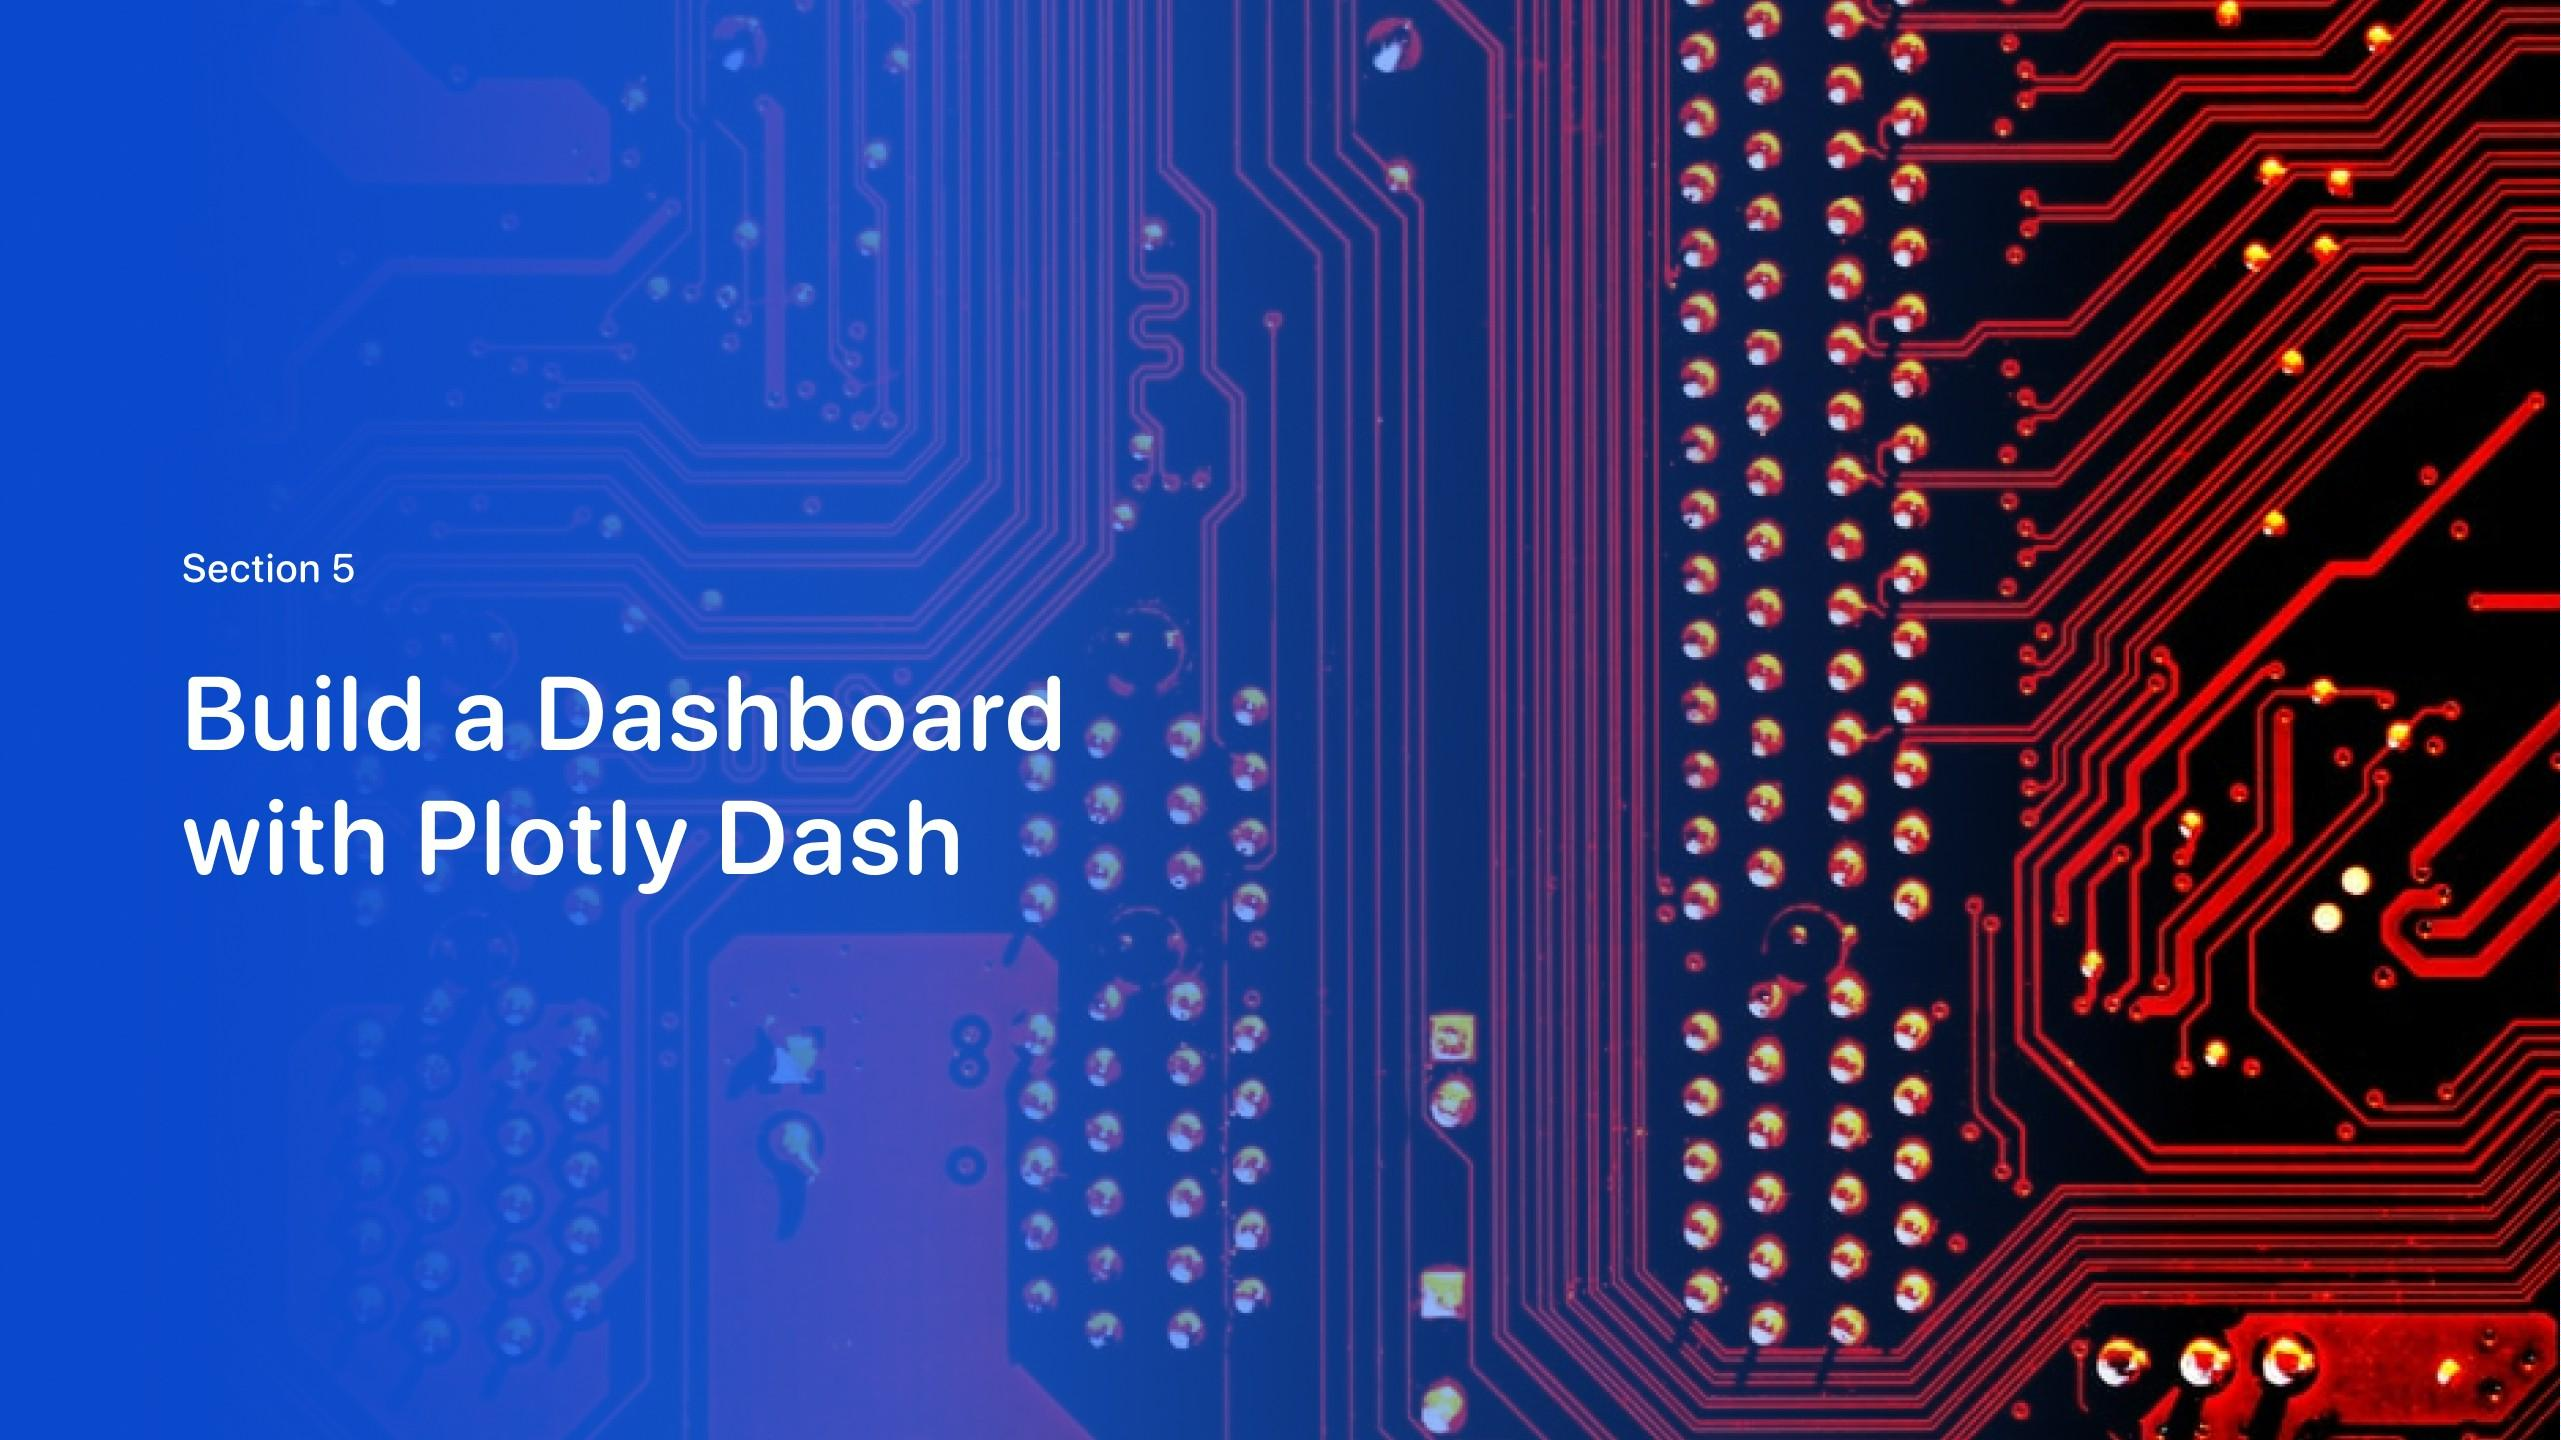
\includegraphics[width=960.009pt,height=540pt]{latexImage_6119fa1a037d088c25bad92d086ab731.png}}
\end{picture}
\begin{tikzpicture}[overlay]
\path(0pt,0pt);
\filldraw[color_40875][even odd rule]
(88.493pt, -217.877pt) -- (47.844pt, -217.877pt)
 -- (47.844pt, -217.877pt)
 -- (47.844pt, -189.162pt)
 -- (47.844pt, -189.162pt)
 -- (129.142pt, -189.162pt)
 -- (129.142pt, -189.162pt)
 -- (129.142pt, -217.877pt)
 -- (129.142pt, -217.877pt)
 -- (88.493pt, -217.877pt) -- cycle
;
\end{tikzpicture}
\begin{picture}(-5,0)(2.5,0)
\put(54.902,-210.706){\fontsize{18}{1}\usefont{T1}{cmr}{m}{n}\selectfont\color{color_283006}Section 4}
\end{picture}
\newpage
\begin{tikzpicture}[overlay]
\path(0pt,0pt);
\filldraw[color_283006][even odd rule]
(-15pt, 10pt) -- (944.981pt, 10pt)
 -- (944.981pt, 10pt)
 -- (944.981pt, -529.972pt)
 -- (944.981pt, -529.972pt)
 -- (-15pt, -529.972pt)
 -- (-15pt, -529.972pt)
 -- (-15pt, 10pt) -- cycle
;
\end{tikzpicture}
\begin{picture}(-5,0)(2.5,0)
\put(-15,-529.972){
\includegraphics[width=960.009pt,height=540.0001pt]{latexImage_bc4b5025d16a0dea794d2300a0dfe378.png}}
\put(859.602,-486.687){\fontsize{15.987}{1}\usefont{T1}{cmr}{m}{n}\selectfont\color{color_60793}39}
\put(52.805,-159.313){\fontsize{21.997}{1}\usefont{T1}{cmr}{m}{n}\selectfont\color{color_70504}Replace <Dashboard screenshot 1> title with an appropriate title}
\put(52.805,-239.987){\fontsize{21.997}{1}\usefont{T1}{cmr}{m}{n}\selectfont\color{color_70504}Show the screenshot of launch success count for all sites, in a }
\put(52.805,-266.406){\fontsize{21.997}{1}\usefont{T1}{cmr}{m}{n}\selectfont\color{color_70504}piechart}
\put(52.805,-347.109){\fontsize{21.997}{1}\usefont{T1}{cmr}{m}{n}\selectfont\color{color_70504}Explain the important elements and findings on the screenshot}
\put(52.805,-64.69299){\fontsize{33.194}{1}\usefont{T1}{cmr}{m}{n}\selectfont\color{color_42828}<Dashboard Screenshot 1>}
\end{picture}
\newpage
\begin{tikzpicture}[overlay]
\path(0pt,0pt);
\filldraw[color_283006][even odd rule]
(-15pt, 10pt) -- (944.981pt, 10pt)
 -- (944.981pt, 10pt)
 -- (944.981pt, -529.972pt)
 -- (944.981pt, -529.972pt)
 -- (-15pt, -529.972pt)
 -- (-15pt, -529.972pt)
 -- (-15pt, 10pt) -- cycle
;
\end{tikzpicture}
\begin{picture}(-5,0)(2.5,0)
\put(-15,-529.972){
\includegraphics[width=960.009pt,height=540.0001pt]{latexImage_bc4b5025d16a0dea794d2300a0dfe378.png}}
\put(859.602,-486.687){\fontsize{15.987}{1}\usefont{T1}{cmr}{m}{n}\selectfont\color{color_60793}40}
\put(49.998,-159.313){\fontsize{21.997}{1}\usefont{T1}{cmr}{m}{n}\selectfont\color{color_70504}Replace <Dashboard screenshot 2> title with an appropriate title}
\put(49.998,-239.987){\fontsize{21.997}{1}\usefont{T1}{cmr}{m}{n}\selectfont\color{color_70504}Show the screenshot of the piechart for the launch site with highest }
\put(49.998,-266.406){\fontsize{21.997}{1}\usefont{T1}{cmr}{m}{n}\selectfont\color{color_70504}launch success ratio}
\put(49.998,-347.109){\fontsize{21.997}{1}\usefont{T1}{cmr}{m}{n}\selectfont\color{color_70504}Explain the important elements and findings on the screenshot}
\put(52.805,-64.69299){\fontsize{33.194}{1}\usefont{T1}{cmr}{m}{n}\selectfont\color{color_42828}<Dashboard Screenshot 2>}
\end{picture}
\newpage
\begin{tikzpicture}[overlay]
\path(0pt,0pt);
\filldraw[color_283006][even odd rule]
(-15pt, 10pt) -- (944.981pt, 10pt)
 -- (944.981pt, 10pt)
 -- (944.981pt, -529.972pt)
 -- (944.981pt, -529.972pt)
 -- (-15pt, -529.972pt)
 -- (-15pt, -529.972pt)
 -- (-15pt, 10pt) -- cycle
;
\end{tikzpicture}
\begin{picture}(-5,0)(2.5,0)
\put(-15,-529.972){
\includegraphics[width=960.009pt,height=540.0001pt]{latexImage_bc4b5025d16a0dea794d2300a0dfe378.png}}
\put(859.602,-486.687){\fontsize{15.987}{1}\usefont{T1}{cmr}{m}{n}\selectfont\color{color_60793}41}
\put(52.805,-159.313){\fontsize{21.997}{1}\usefont{T1}{cmr}{m}{n}\selectfont\color{color_70504}Replace <Dashboard screenshot 3> title with an appropriate title}
\put(52.805,-239.987){\fontsize{21.997}{1}\usefont{T1}{cmr}{m}{n}\selectfont\color{color_70504}Show screenshots of Payload vs. Launch Outcome scatter plot for all }
\put(52.805,-266.406){\fontsize{21.997}{1}\usefont{T1}{cmr}{m}{n}\selectfont\color{color_70504}sites, with different payload selected in the range slider}
\put(52.805,-347.109){\fontsize{21.997}{1}\usefont{T1}{cmr}{m}{n}\selectfont\color{color_70504}Explain the important elements and findings on the screenshot, such as }
\put(52.805,-373.499){\fontsize{21.997}{1}\usefont{T1}{cmr}{m}{n}\selectfont\color{color_70504}which payload range or booster version have the largest success rate, }
\put(52.805,-399.89){\fontsize{21.997}{1}\usefont{T1}{cmr}{m}{n}\selectfont\color{color_70504}etc.}
\put(52.805,-64.69299){\fontsize{33.194}{1}\usefont{T1}{cmr}{m}{n}\selectfont\color{color_42828}<Dashboard Screenshot 3>}
\end{picture}
\newpage
\begin{tikzpicture}[overlay]
\path(0pt,0pt);
\filldraw[color_283006][even odd rule]
(-15pt, 10pt) -- (944.981pt, 10pt)
 -- (944.981pt, 10pt)
 -- (944.981pt, -529.972pt)
 -- (944.981pt, -529.972pt)
 -- (-15pt, -529.972pt)
 -- (-15pt, -529.972pt)
 -- (-15pt, 10pt) -- cycle
;
\end{tikzpicture}
\begin{picture}(-5,0)(2.5,0)
\put(-15,-529.972){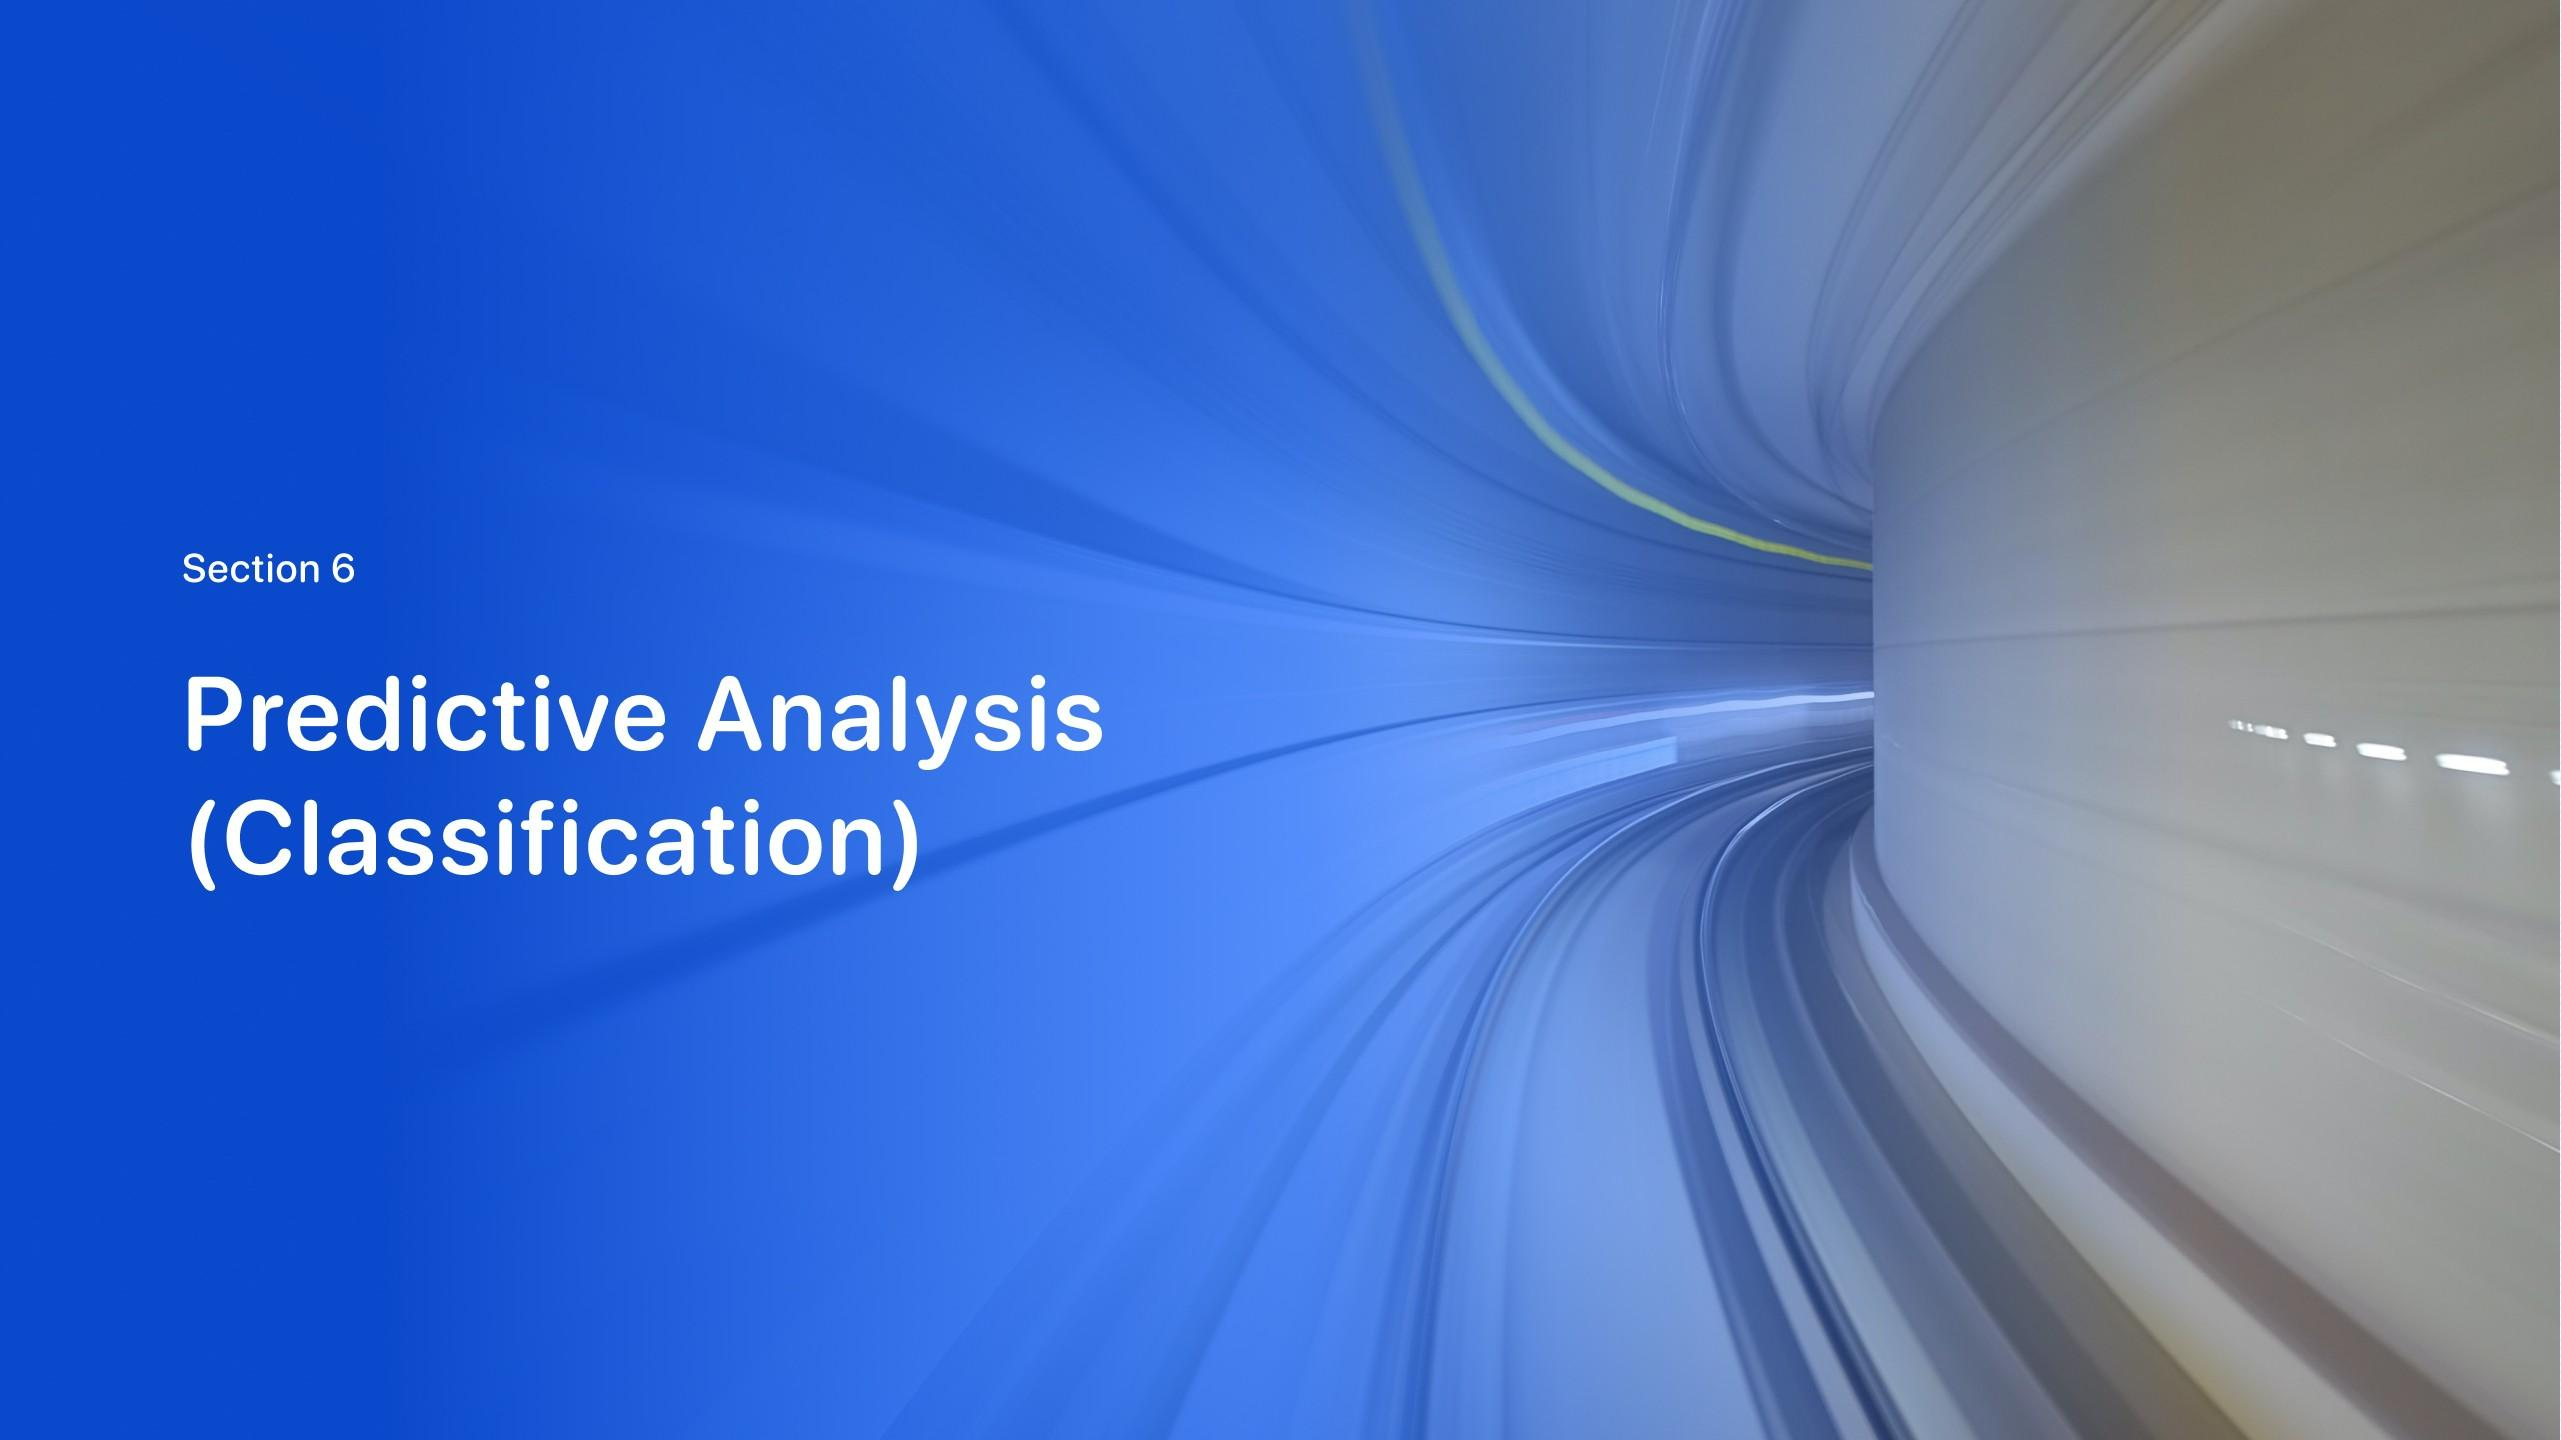
\includegraphics[width=960.009pt,height=540pt]{latexImage_650b44f4ee0b3aaf8230a3a4a0bb9be3.png}}
\end{picture}
\begin{tikzpicture}[overlay]
\path(0pt,0pt);
\filldraw[color_40875][even odd rule]
(88.493pt, -217.877pt) -- (47.844pt, -217.877pt)
 -- (47.844pt, -217.877pt)
 -- (47.844pt, -189.162pt)
 -- (47.844pt, -189.162pt)
 -- (129.142pt, -189.162pt)
 -- (129.142pt, -189.162pt)
 -- (129.142pt, -217.877pt)
 -- (129.142pt, -217.877pt)
 -- (88.493pt, -217.877pt) -- cycle
;
\end{tikzpicture}
\begin{picture}(-5,0)(2.5,0)
\put(54.902,-210.706){\fontsize{18}{1}\usefont{T1}{cmr}{m}{n}\selectfont\color{color_283006}Section 5}
\end{picture}
\newpage
\begin{tikzpicture}[overlay]
\path(0pt,0pt);
\filldraw[color_283006][even odd rule]
(-15pt, 10pt) -- (944.981pt, 10pt)
 -- (944.981pt, 10pt)
 -- (944.981pt, -529.972pt)
 -- (944.981pt, -529.972pt)
 -- (-15pt, -529.972pt)
 -- (-15pt, -529.972pt)
 -- (-15pt, 10pt) -- cycle
;
\end{tikzpicture}
\begin{picture}(-5,0)(2.5,0)
\put(-15,-529.972){
\includegraphics[width=960.009pt,height=540.0001pt]{latexImage_bc4b5025d16a0dea794d2300a0dfe378.png}}
\put(859.602,-486.687){\fontsize{15.987}{1}\usefont{T1}{cmr}{m}{n}\selectfont\color{color_60793}43}
\put(52.805,-178.391){\fontsize{21.997}{1}\usefont{T1}{cmr}{m}{n}\selectfont\color{color_70504}•}
\put(70.805,-179.496){\fontsize{21.997}{1}\usefont{T1}{cmr}{m}{n}\selectfont\color{color_70504}Visualize the built model accuracy }
\put(70.805,-205.887){\fontsize{21.997}{1}\usefont{T1}{cmr}{m}{n}\selectfont\color{color_70504}for all built classification models, }
\put(70.805,-232.192){\fontsize{21.997}{1}\usefont{T1}{cmr}{m}{n}\selectfont\color{color_70504}in a bar chart}
\put(52.805,-311.789){\fontsize{21.997}{1}\usefont{T1}{cmr}{m}{n}\selectfont\color{color_70504}•}
\put(70.805,-313.008){\fontsize{21.997}{1}\usefont{T1}{cmr}{m}{n}\selectfont\color{color_70504}Find which model has the highest }
\put(70.805,-339.313){\fontsize{21.997}{1}\usefont{T1}{cmr}{m}{n}\selectfont\color{color_70504}classification accuracy}
\put(52.805,-64.69299){\fontsize{33.194}{1}\usefont{T1}{cmr}{m}{n}\selectfont\color{color_42828}Classification Accuracy}
\end{picture}
\newpage
\begin{tikzpicture}[overlay]
\path(0pt,0pt);
\filldraw[color_283006][even odd rule]
(-15pt, 10pt) -- (944.981pt, 10pt)
 -- (944.981pt, 10pt)
 -- (944.981pt, -529.972pt)
 -- (944.981pt, -529.972pt)
 -- (-15pt, -529.972pt)
 -- (-15pt, -529.972pt)
 -- (-15pt, 10pt) -- cycle
;
\end{tikzpicture}
\begin{picture}(-5,0)(2.5,0)
\put(-15,-529.972){
\includegraphics[width=960.009pt,height=540.0001pt]{latexImage_bc4b5025d16a0dea794d2300a0dfe378.png}}
\put(859.602,-486.687){\fontsize{15.987}{1}\usefont{T1}{cmr}{m}{n}\selectfont\color{color_60793}44}
\put(52.691,-176.293){\fontsize{21.997}{1}\usefont{T1}{cmr}{m}{n}\selectfont\color{color_70504}•}
\put(70.691,-177.512){\fontsize{21.997}{1}\usefont{T1}{cmr}{m}{n}\selectfont\color{color_70504}Show the confusion matrix of the best performing model with an }
\put(70.691,-203.902){\fontsize{21.997}{1}\usefont{T1}{cmr}{m}{n}\selectfont\color{color_70504}explanation }
\put(52.805,-64.69299){\fontsize{33.194}{1}\usefont{T1}{cmr}{m}{n}\selectfont\color{color_42828}Confusion Matrix}
\end{picture}
\newpage
\begin{tikzpicture}[overlay]
\path(0pt,0pt);
\filldraw[color_283006][even odd rule]
(-15pt, 10pt) -- (944.981pt, 10pt)
 -- (944.981pt, 10pt)
 -- (944.981pt, -529.972pt)
 -- (944.981pt, -529.972pt)
 -- (-15pt, -529.972pt)
 -- (-15pt, -529.972pt)
 -- (-15pt, 10pt) -- cycle
;
\end{tikzpicture}
\begin{picture}(-5,0)(2.5,0)
\put(-15,-529.972){
\includegraphics[width=960.009pt,height=540.0001pt]{latexImage_bc4b5025d16a0dea794d2300a0dfe378.png}}
\put(859.602,-486.687){\fontsize{15.987}{1}\usefont{T1}{cmr}{m}{n}\selectfont\color{color_60793}45}
\put(52.691,-163.112){\fontsize{21.997}{1}\usefont{T1}{cmr}{m}{n}\selectfont\color{color_70504}Point 1}
\put(52.691,-203.506){\fontsize{21.997}{1}\usefont{T1}{cmr}{m}{n}\selectfont\color{color_70504}Point 2}
\put(52.691,-243.899){\fontsize{21.997}{1}\usefont{T1}{cmr}{m}{n}\selectfont\color{color_70504}Point 3}
\put(52.691,-284.208){\fontsize{21.997}{1}\usefont{T1}{cmr}{m}{n}\selectfont\color{color_70504}Point 4}
\put(52.691,-324.602){\fontsize{21.997}{1}\usefont{T1}{cmr}{m}{n}\selectfont\color{color_70504}…}
\put(52.805,-64.69299){\fontsize{33.194}{1}\usefont{T1}{cmr}{m}{n}\selectfont\color{color_42828}Conclusions}
\end{picture}
\newpage
\begin{tikzpicture}[overlay]
\path(0pt,0pt);
\filldraw[color_283006][even odd rule]
(-15pt, 10pt) -- (944.981pt, 10pt)
 -- (944.981pt, 10pt)
 -- (944.981pt, -529.972pt)
 -- (944.981pt, -529.972pt)
 -- (-15pt, -529.972pt)
 -- (-15pt, -529.972pt)
 -- (-15pt, 10pt) -- cycle
;
\end{tikzpicture}
\begin{picture}(-5,0)(2.5,0)
\put(-15,-529.972){
\includegraphics[width=960.009pt,height=540.0001pt]{latexImage_bc4b5025d16a0dea794d2300a0dfe378.png}}
\put(859.602,-486.687){\fontsize{15.987}{1}\usefont{T1}{cmr}{m}{n}\selectfont\color{color_60793}46}
\put(52.691,-161.893){\fontsize{21.997}{1}\usefont{T1}{cmr}{m}{n}\selectfont\color{color_70504}Include any relevant assets like Python code snippets, SQL queries, }
\put(52.691,-188.312){\fontsize{21.997}{1}\usefont{T1}{cmr}{m}{n}\selectfont\color{color_70504}charts, Notebook outputs, or data sets that you may have created during }
\put(52.691,-214.589){\fontsize{21.997}{1}\usefont{T1}{cmr}{m}{n}\selectfont\color{color_70504}this project}
\put(52.805,-64.69299){\fontsize{33.194}{1}\usefont{T1}{cmr}{m}{n}\selectfont\color{color_42828}Appendix}
\end{picture}
\newpage
\begin{tikzpicture}[overlay]
\path(0pt,0pt);
\filldraw[color_283006][even odd rule]
(-15pt, 10pt) -- (944.981pt, 10pt)
 -- (944.981pt, 10pt)
 -- (944.981pt, -529.972pt)
 -- (944.981pt, -529.972pt)
 -- (-15pt, -529.972pt)
 -- (-15pt, -529.972pt)
 -- (-15pt, 10pt) -- cycle
;
\end{tikzpicture}
\begin{picture}(-5,0)(2.5,0)
\put(-15,-529.972){\includegraphics[width=960.009pt,height=540pt]{latexImage_6191149a144d91808ade5f0c176cae09.png}}
\end{picture}
\end{document}